%%%%%%%%%%%%%%%%%%%%%%%%%%%%%%%%%%%%%%%%%%%%%%%%%%%%%%%%%%%%%%%
\section{PD Design}
\label{sec:fdsp-pd-design}
%\metainfo{(Length: TDR=50 pages, TP=20 pages)}
%\metainfo{\color{blue} Content: Conveners}

%dww edits 16mar18
%rjw edits 15mar18

%\fixme{Include an image of the subsystem, indicating its parts. Show how the system fits into the overall system).}

The core modular element of the PD system are the large area {\it photon collectors} that convert incident \SI{128}{nm} scintillation photons into photon in the visible range (>\SI{400}{nm}), which in turn are converted to an electrical signal by compact silicon photomultipliers (SiPM) {\it photon sensors}. At the time of the Technical Proposal there are three photon collector options under consideration; figure~\ref{fig:3dtpc-pd} shows how they are incorporated into the TPC anode plane assembly by an identical mounting scheme. In the following we summarize the design and development status for each photon collector option. 
[For the Technical Design Report there will be a baseline design and at most one alternative.]

%%%%%%%%%%%%%%%%%%%%%%%%%%%%%%%%%%%
%\subsection{Photon Collector}
%\label{sec:fdsp-pd-pc}
%\metainfo{\color{blue} Content: Cavanna/Whittington/Machado}


%==================================================================================================================
% We need a neutrino detection efficiency for all the options - perhaps this should be in a separate Physics Performance  section.
%
%The response of this module has been simulated within the DUNE single-phase far detector module. Low-energy neutrinos from a galactic core-collapse 
%supernova represent one of the most challenging physics channels for the photon detection system. Figure~\ref{fig:pds-sn-eff-simulation} shows the 
%preliminary neutrino detection efficiency versus energy of the electron produced in the neutrino interaction for a variety of relative efficiencies of the double-
%shift light guide detector. The simulation of the performance described above results in the efficiency curve labeled ``standard'' and results in an average 
%efficiency for the photon detection system to unambiguously reconstruct the neutrino interaction time between 30\% at 5~MeV and 70\% at 15~MeV of visible 
%energy.

%\begin{dunefigure}[Neutrino detection efficiency.]
%{fig:pds-sn-eff-simulation}
%{Preliminary neutrino detection efficiency versus energy of the electron produced in the neutrino interaction for a variety of relative efficiencies of the double-%shift light guide detector. The curve marked ``standard'' represents performance described in the text.} 
%\includegraphics[width=0.5\columnwidth]{pds-sn-eff-%simulation.png}
%\end{dunefigure}
%==================================================================================================================

%%%%
% Moved to the overview section. rjw
%A factor of two improvement in the effective area of the double-shift light guide module provides two benefits. The efficiency to identify the interaction time 
%(and subsequently improve the calorimetric energy resolution of the interaction through drift-distance correction) is substantially improved at all energies. 
%Perhaps more importantly, the supernova neutrino tagging efficiency is more robust against uncertainty in the final module performance and manufacturing 
%variations between modules once the light collector efficiency is 2.0$\times$ standard or greater.

%DWW 16mar18 start %%%%%%

%moved below the double shift section

%\subsubsection{Potential Improvements for final design}

%The double-shift light guide deployed in the ProtoDUNE-SP APAs was constrained to readout at a single end. Proposed changes to the APA size %and cabling routing scheme for the DUNE single-phase far detector would allow for a second array of SiPMs at the opposite end of the light %guide. This would double the performance of the photon detection system, raising the per-module effective area to 8.2 cm$^{2}$ per module %per drift volume.

%A SiPM with a wavelength-dependent PDE that is better matched to the EJ-280 emission spectrum would improve the overall efficiency. %Simulations of the transport of light within the light guide suggest that applying a highly reflective coating to the long, narrow inactive %sides of the light guide would further boost the attenuation function and increase the effective area of the light guide module. These %effects combined lead to a potential increase of the effective area to 16 cm$^{2}$ per module per drift volume.

%As is illustrated in Figure~\ref{fig:pds-sn-eff-simulation}, the simulated supernova neutrino detection capability of a photon detection %system based on this %module depends strongly on small changes in the estimated efficiency. These potential improvements raise the physics %performance in this channel into a %regime where small fluctuations in the module efficiency have a smaller impact on the efficiency to tag %these supernova neutrino interactions. These %improvements are an important component to risk mitigation in the photon detection system %performance.

%DWW 15mar18 end %%%%%%

\subsection{Photon Collector: ARAPUCA}
\label{ssec:fdsp-pd-pc-arapuca}
%\todo{\color{blue} Content: A.Machado}

%\fixme{Does not have bibliography  integrated yet.}

The ARAPUCA is a device based on a new approach to liquid argon scintillation photon detection.  The basic concept of the ARAPUCA is to trap photons inside a box with highly reflective internal surfaces until reflections guide them to an SiPM, so that the detection efficiency of trapped photons is high even with a limited active coverage of its internal surface \cite{arapuca_jinst}. It provides a large area window (tens of \si{cm$^2$} with detection efficiencies of several percent while using a coverage with active devices (SiPMs) at the part per-mil level.

Photon trapping is achieved by using a smart wave-shifting technique and the technology of the dichroic shortpass optical filters. The latter are multilayer thin films with the property of being highly transparent to photons with a wavelength below a tunable cut-off while being almost perfectly reflective to photons with wavelength above the cut-off. A dichroic shortpass filter deposited with one or two different wavelength shifters (either only on the outside face or one on each side) will be the acceptance window of the ARAPUCA. The rest of the device will be a flattened box with internal surfaces covered by highly reflective acrylic foils (3M-Vikuiti ESR \cite{Vikuiti}, for example), closed on the top by the dichroic filter acceptance window. In principle the box can be filled with any kind of transparent material, since it is not essential to its operation. A fraction of the box internal surface is occupied by the active photosensors (SiPM) that detect trapped photons.

\subsubsection{Operating principle}
The operating principle for ARAPUCA is quite straightforward. The wavelength-shifter deposited on the outer face of the dichroic filter, and that on the inside of the box (S$_1$ and S$_2$ respectively), must have their emission wavelengths, L$_1$ and L$_2$, such that: L$_1$ $<$ L$_{cut-off}$$ <$ L$_2$, where L$_{cut-off}$ is the cut-off wavelength of the filter, that is the limit between the region of full transparency (typically $>$ 95\%) and that of full reflectivity (typically $>$ 98\%). The coated surface deposited with S$_2$ faces the internal part of the box (a variant of the concept place the second wavelength-shifter on highly-reflective surfaces inside the box).

In a LAr volume, a fraction of the scintillation VUV photons ($\lambda \sim$ \SI{127}{nm}) produced by the passage of an ionizing radiation, hit the window of the ARAPUCA and are shifted to a wavelength of L$_1$ by the shifter deposited on the external face of the filter and a significant fraction travel towards the internal cavity of the ARAPUCA. On the coated surface inside the box the photons are converted to the wavelength L$_2$ and so are effectively trapped inside the box since the internal surface of the box is covered with a very high reflectance material in this wavelength range and the filter that forms the one-way window into  the box is itself reflective to L$_2$ photons.  After a few reflections the photons are detected by the SiPM installed on the internal surface of the ARAPUCA (Figure \ref{arapuca}). 

The net effect of the ARAPUCA is to amplify the active area of the SiPM used to readout the trapped photons. It is easy to show that for small values of SiPM coverage of the internal surface the amplification factor is equal to $A=1/2(1-R)$,
%\begin{equation}
%A=\frac{1}{2(1-R)}
%\end{equation}
where R is the average value of the reflectivity of the internal surfaces. For an average reflectivity of 0.95 the amplification factor is equal to ten.

\begin{dunefigure}[ARAPUCA and the schematic representation of the operating principle.]{fig:arapuca}
{ARAPUCA and the schematic representation of the operating principle.}
  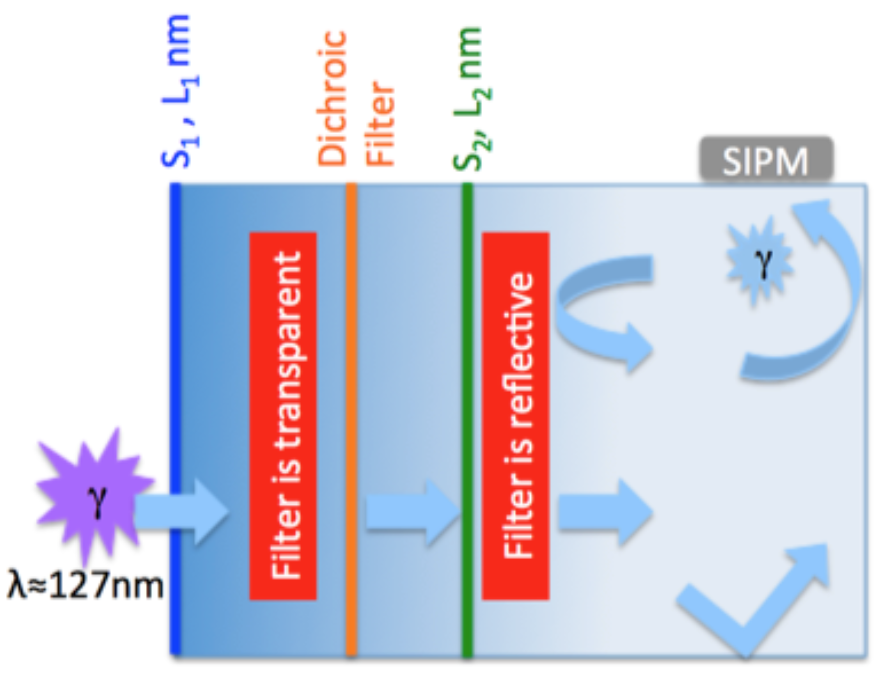
\includegraphics[height=5cm]{pds-arpkscheme}   
\end{dunefigure}

In the next sections we describe a variety of tests of the technology performed at three primary locations.

\subsubsection{Tests performed in Brazil}
\label{subsec:testlnls}

Tests of the ARAPUCA in a liquid argon (LAr) environment were performed at the facilities of the Toroidal Grating Monochromator (TGM) beamline of the Brazilian Synchrotron Light Laboratory (LNLS) (Figure \ref{LNLS_test}). 

A small ARAPUCA made of PTFE with internal dimensions of 3.5~x~2.5~x~0.6~cm$^3$ was tested and a dichroic filter with dimensions of 3.5~x~2.5~cm$^2$ and cut-off at 400 nm was used as the window of the device.
The filter was evaporated with p-TerPhenyl (pTP), which absorbs 127 nm photons and reemits them around 350 nm,  on the external side and TetraPhenyl-Butadiene (TPB) on the internal side, which absorbs the shifted 350 nm photons and reemits around 430 nm. Trapped light was detected by a single 0.6~x~0.6~cm$^2$  SensL SiPMs mod C60035.
The device was installed inside a vacuum tight stainless-steel cylinder closed by two CF100 flanges. The cylinder was deployed inside a LAr open bath, vacuum pumped down to a pressure around  10$^{-6}$ mbar and then filled with one liter of ultra pure liquid argon. 

LAr scintillation light emission was produced by an alpha source installed in front of the ARAPUCA, immersed in liquid argon. Signals were read-out through an Aquiris\footnote{Aquiris High-Speed Digitizer products http://www.acqiris.com/} PCI board and stored on a computer.

%*****************************FIGURE 3*****************************%
\begin{dunefigure}[ARAPUCA test at LNLS]{LNLS_test}
{ARAPUCA test at LNLS} 
	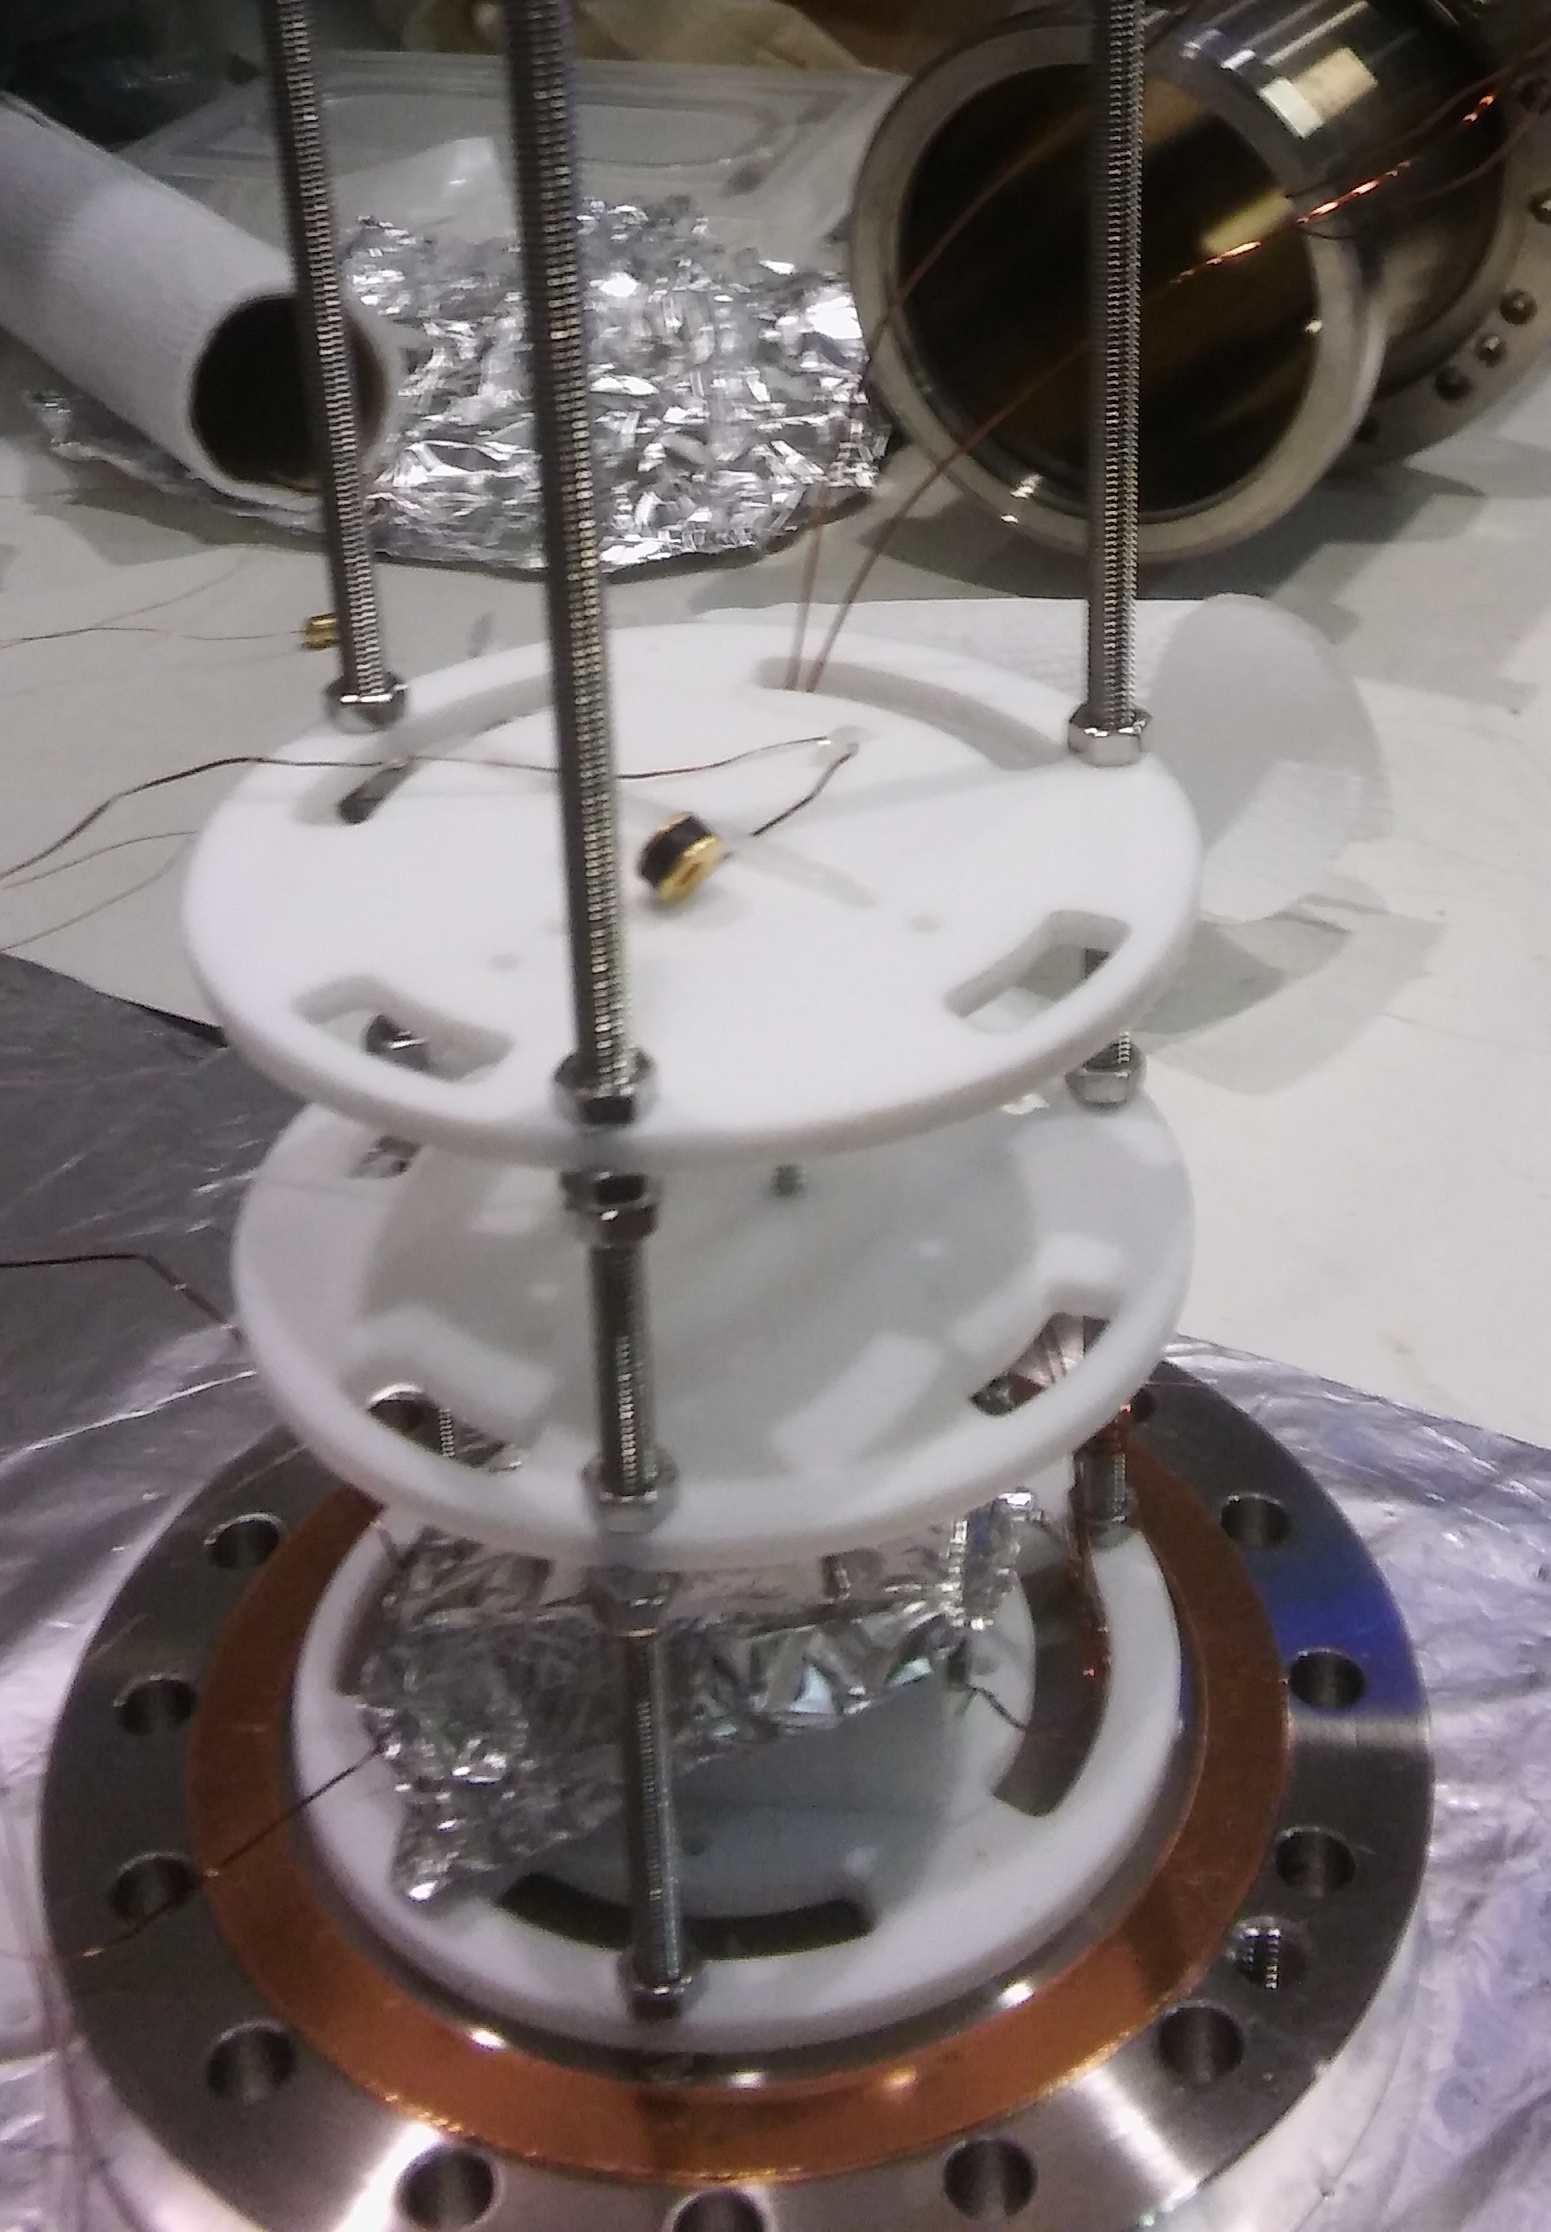
\includegraphics[height=5cm]{pds-tgm_1} \quad
	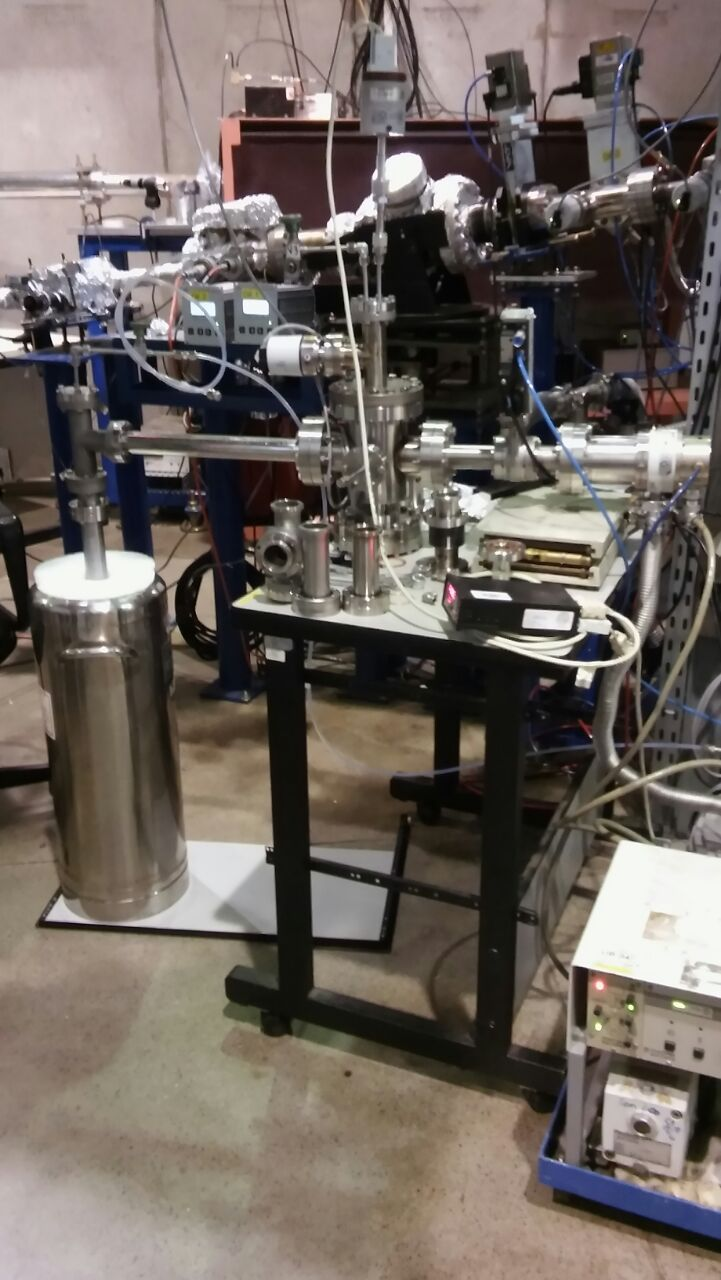
\includegraphics[height=5cm]{pds-tgm_30}\quad
	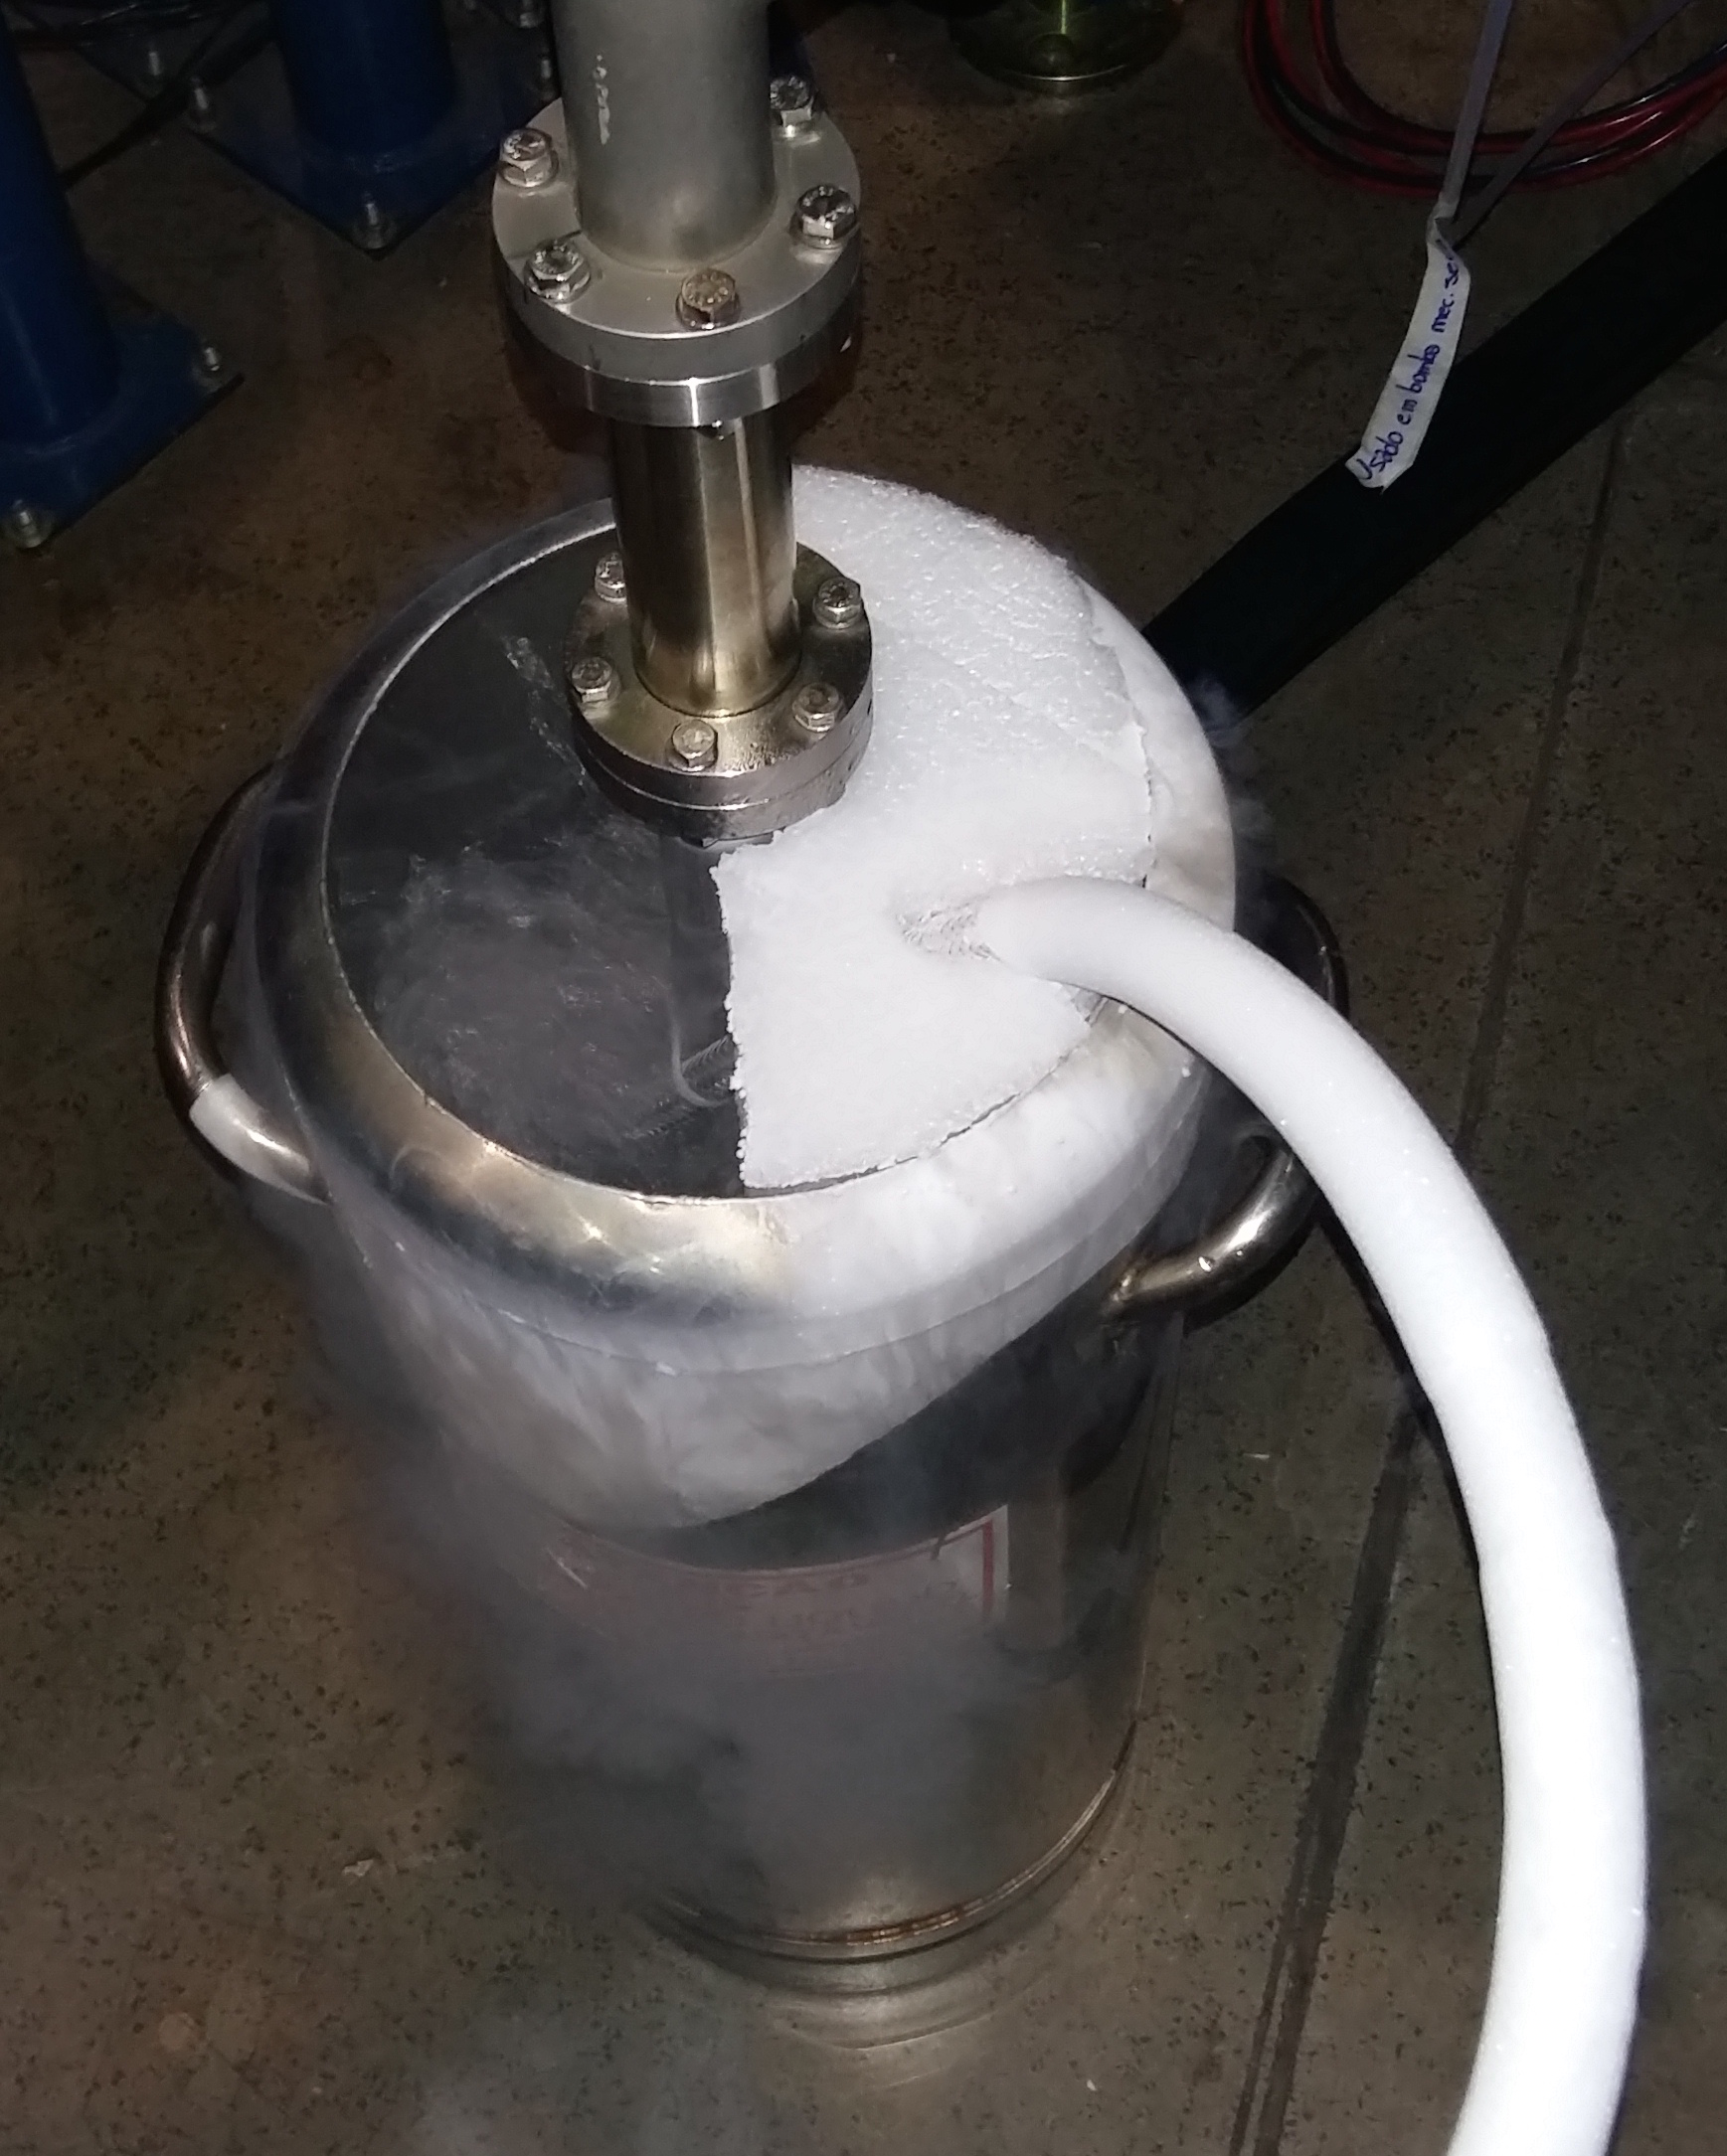
\includegraphics[height=5cm]{pds-tgm_0}
%\fixme{Missing three figures \texttt{pds-tgm*}.} -- found rjw
\end{dunefigure}
%***********************************************************************%

It was possible to estimate the detection efficiency of the ARAPUCA by 
determining the number of photoelectrons detected corresponding to the end point of the $\alpha$ spectrum 
and comparing it with the expected number of photons impinging on the acceptance window for that 
particular energy value ($\sim$ 4.3 MeV), which depends only on known properties of LAr and on the solid 
angle subtended by the the ARAPUCA window. A detection efficiency at the level of 1.8 \% 
was found,  consistent with Monte Carlo expectations.

\subsubsection{Tests performed at FERMILAB}
\label{subsec:test_fnal}

Three cryogenic tests have been performed at Fermilab:
\begin{itemize}
\item The first  was performed in mid-2016 at the Proton Assembly Building (PAB) at the ScENE cryogenic test facility. The ARAPUCA prototype had dimensions of  $5.0 \times 5.0 \times 1.0$ cm$^3$ with a dichroic window of $5.0 \times 5.0$ cm$^2$ deposited with pTP and TPB, respectively on the internal and external faces. The cut-off of the filter was at 400 nm. Two SensL SiPMs mod C60035 ($0.6 \times 0.6$ cm$^2$ active area each) were installed inside the box to detect trapped photons. 

The ARAPUCA was deployed inside a vacuum tight cryostat filled with ultrapure LAr. An $^{241}$Am alpha source was positioned in front of the window of the device at a distance of 5 cm from its center. The efficiency of the ARAPUCA was estimated taking into account that the alpha particles have a  monochromatic energy of about 5.4 MeV. 
The estimated efficiency in this case was of the order of 1\%, a factor two below what expected likely due to the sub-optimal quality and uniformity of the pTP and TPB films and to the lack of reflectivity of the inner PTFE surfaces.

\item The second  was performed at the beginning of 2017 at the PAB, but using a different facility, 
TallBo, which was large enough to allowed testing of several devices at a time. Eight different ARAPUCAs with 
filters from different manufacturers, different reflectors, and different dimensions were tested. The ARAPUCAs 
were exposed to the 127 nm scintillation light produced by alpha particles emitted by an $^{241}$Am 
source, mounted on a holder that could be moved with an external manipulator in order to place it in 
front of each prototype. The efficiencies of these ARAPUCAs ranged from 0.4\% to 1.0\%.

\item A third test was performed at the end of 2017 with an array of eight ARAPUCAs together with two 
reference bars (double-shift design) in the TallBo set-up. Data analysis is ongoing. 

\end{itemize}

\subsubsection{ARAPUCA in ProtoDUNE-SP}

Two arrays of ARAPUCA modules will be installed inside ProtoDUNE-SP to test the devices in a real experimental environment and to directly compare their performance with those of the guiding bars. The first array has been already installed in the APA \#3, while the second one will be installed in the APA \#6.
 
Each ARAPUCA array is composed of sixteen basic cells. Each cell is an ARAPUCA box with dimensions of 8 cm $\times$ 10 cm and has 12 SiPMs (or 6 SIPMs in some cases) installed on the bottom side of the cell (6 mm $\times$ 6 mm each), as illustrated in Figure \ref{fig:arpk}.
The SiPMs  are passively ganged together, so that only one read-out channel is needed for each ARAPUCA grouping of 12 SiPMs (the boxes with 6 SiPMs are ganged together to form 12-SiPM units) so a total of 12 channels is required per array; studies are underway to investigate {\it active} ganging that would permit combining signals from multiples boxes as required to reduce the number of electronics channels and cables, as needed. 
The ARAPUCA array has a footprint of approximately 8 cm $\times$ 200 cm, the same as the bar wavelength-shifting bars approaches. 
The first ARAPUCA array installed in ProtoDUNE-SP is shown in Figure~\ref{fig:arapuca_array}.

\begin{dunefigure}[Drawing of two ARAPUCAs of the design used for ProtoDUNE-SP.]{fig:arpk}
{Drawing of two ARAPUCAs in one modular unit, each one read-out by 12 SiPMs; this design was used for ProtoDUNE-SP.} 
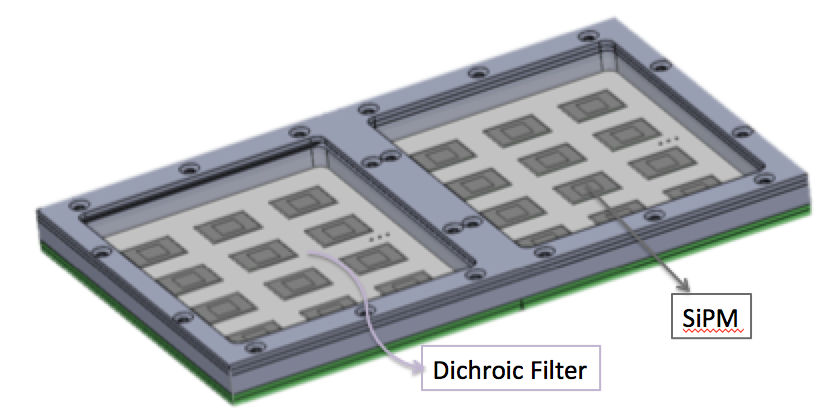
\includegraphics[height=4cm]{pds-arapuca}
\end{dunefigure}


\begin{dunefigure}[ARAPUCA array in ProtoDUNE-SP.]{fig:arapuca_array}
{ARAPUCA array in ProtoDUNE-SP.} 	
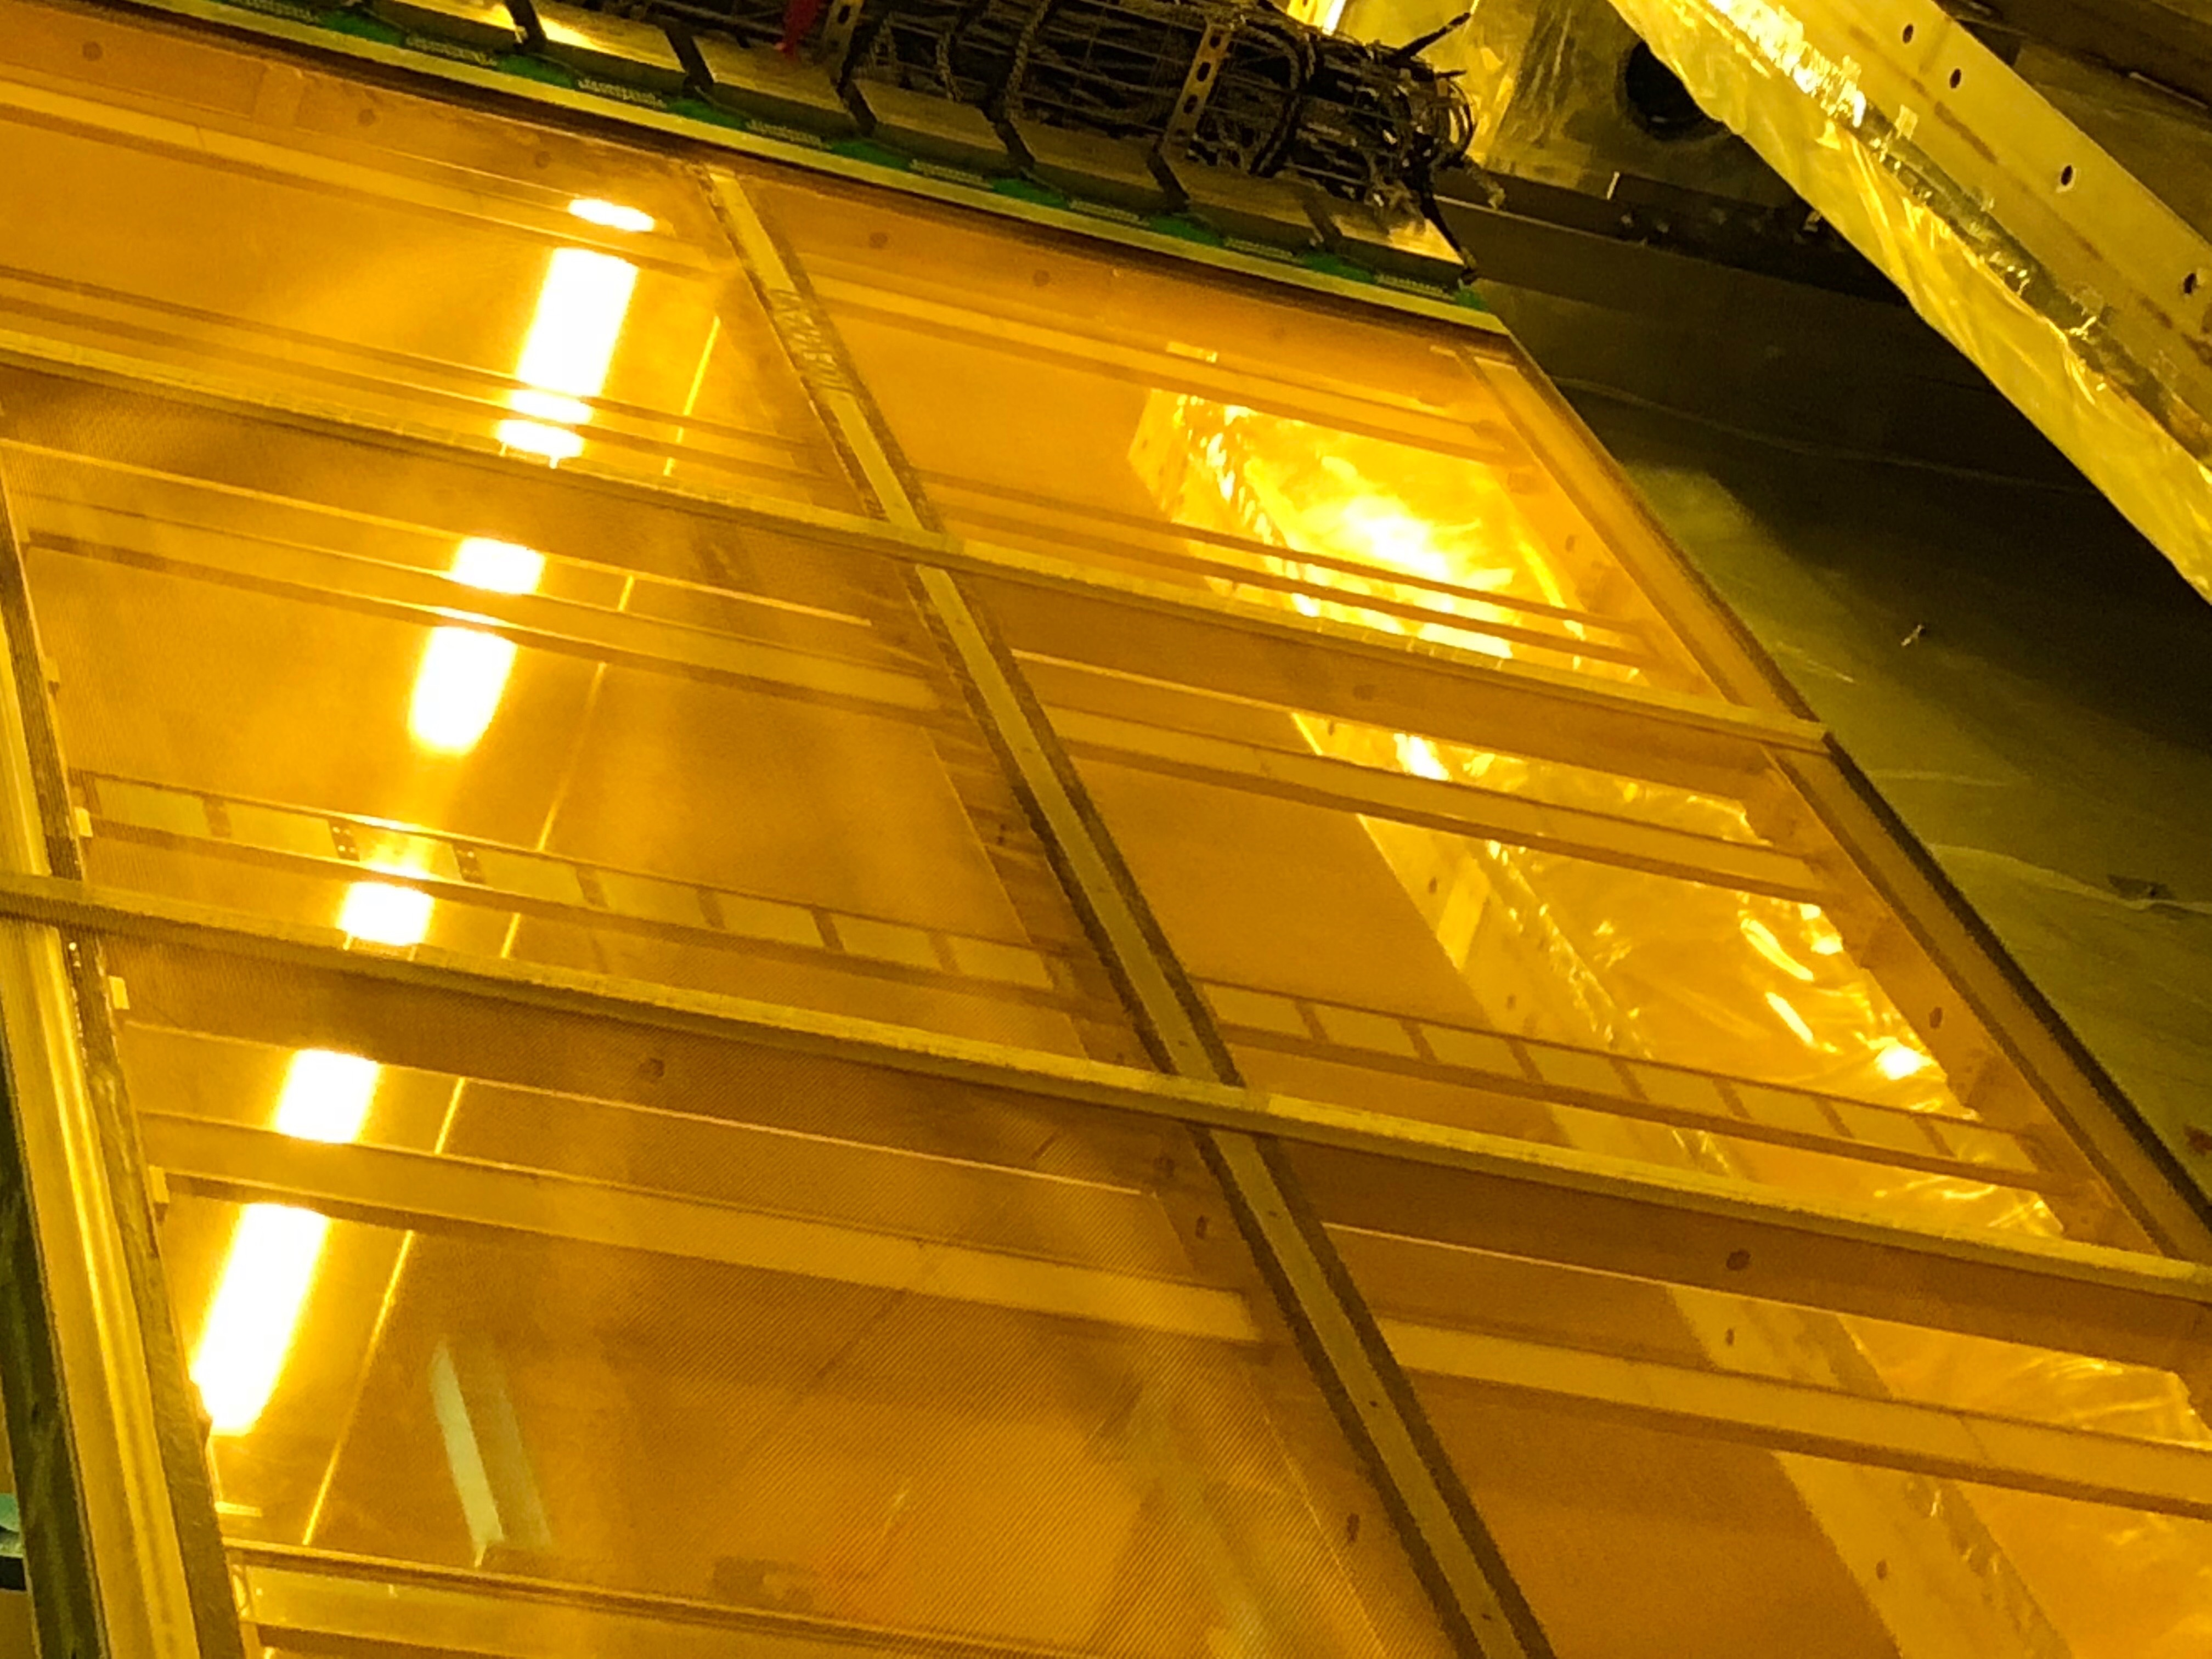
\includegraphics[height=8cm]{pds-arpk-apa3_pd.jpg} 
\end{dunefigure}
%***********************************************************************%

%The ARAPUCA device is undergoing an intense R\&D program that aims to establish its 
%viability as the photon detection system for the single phase DUNE far detector, both 
%in terms of demonstrating an absolute detection efficiency of several percent and with respect to long term reliability.

\subsubsection{X-ARAPUCA}  
X-ARAPUCA represents  an alternate line of development of the ARAPUCA  with the aim of further improving the collection efficiency, while retaining the same working principle, mechanical design and active  photo-sensitive coverage. In a sense X-ARAPUCA is a hybrid solution between the ARAPUCA and the wavelength-shifting light guide bar PDS concepts, where photons trapped in the ARAPUCA box are shifted and transported to the readout via total internal reflection in a light guide placed inside the box.
This solution minimizes the number of reflections on the internal surfaces of the box and thus the probability of photon loss. Simulations suggest that this modification will lead to a rather significant increase of the collection efficiency.

 \begin{dunefigure}[X-ARAPUCA design: assembled cell (left),  exploded view (right).]{fig:pds-x-arapuca-cell}
{X-ARAPUCA design: assembled cell (left),  exploded view (right).}
 % \vspace{-2.5cm}
  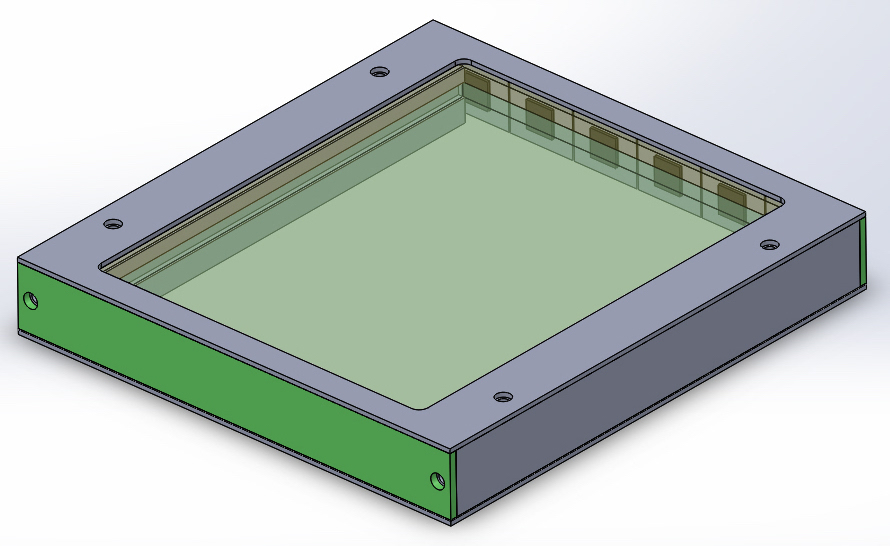
\includegraphics[height=.20\textheight]{pds-x-arapuca-cell.jpg}
  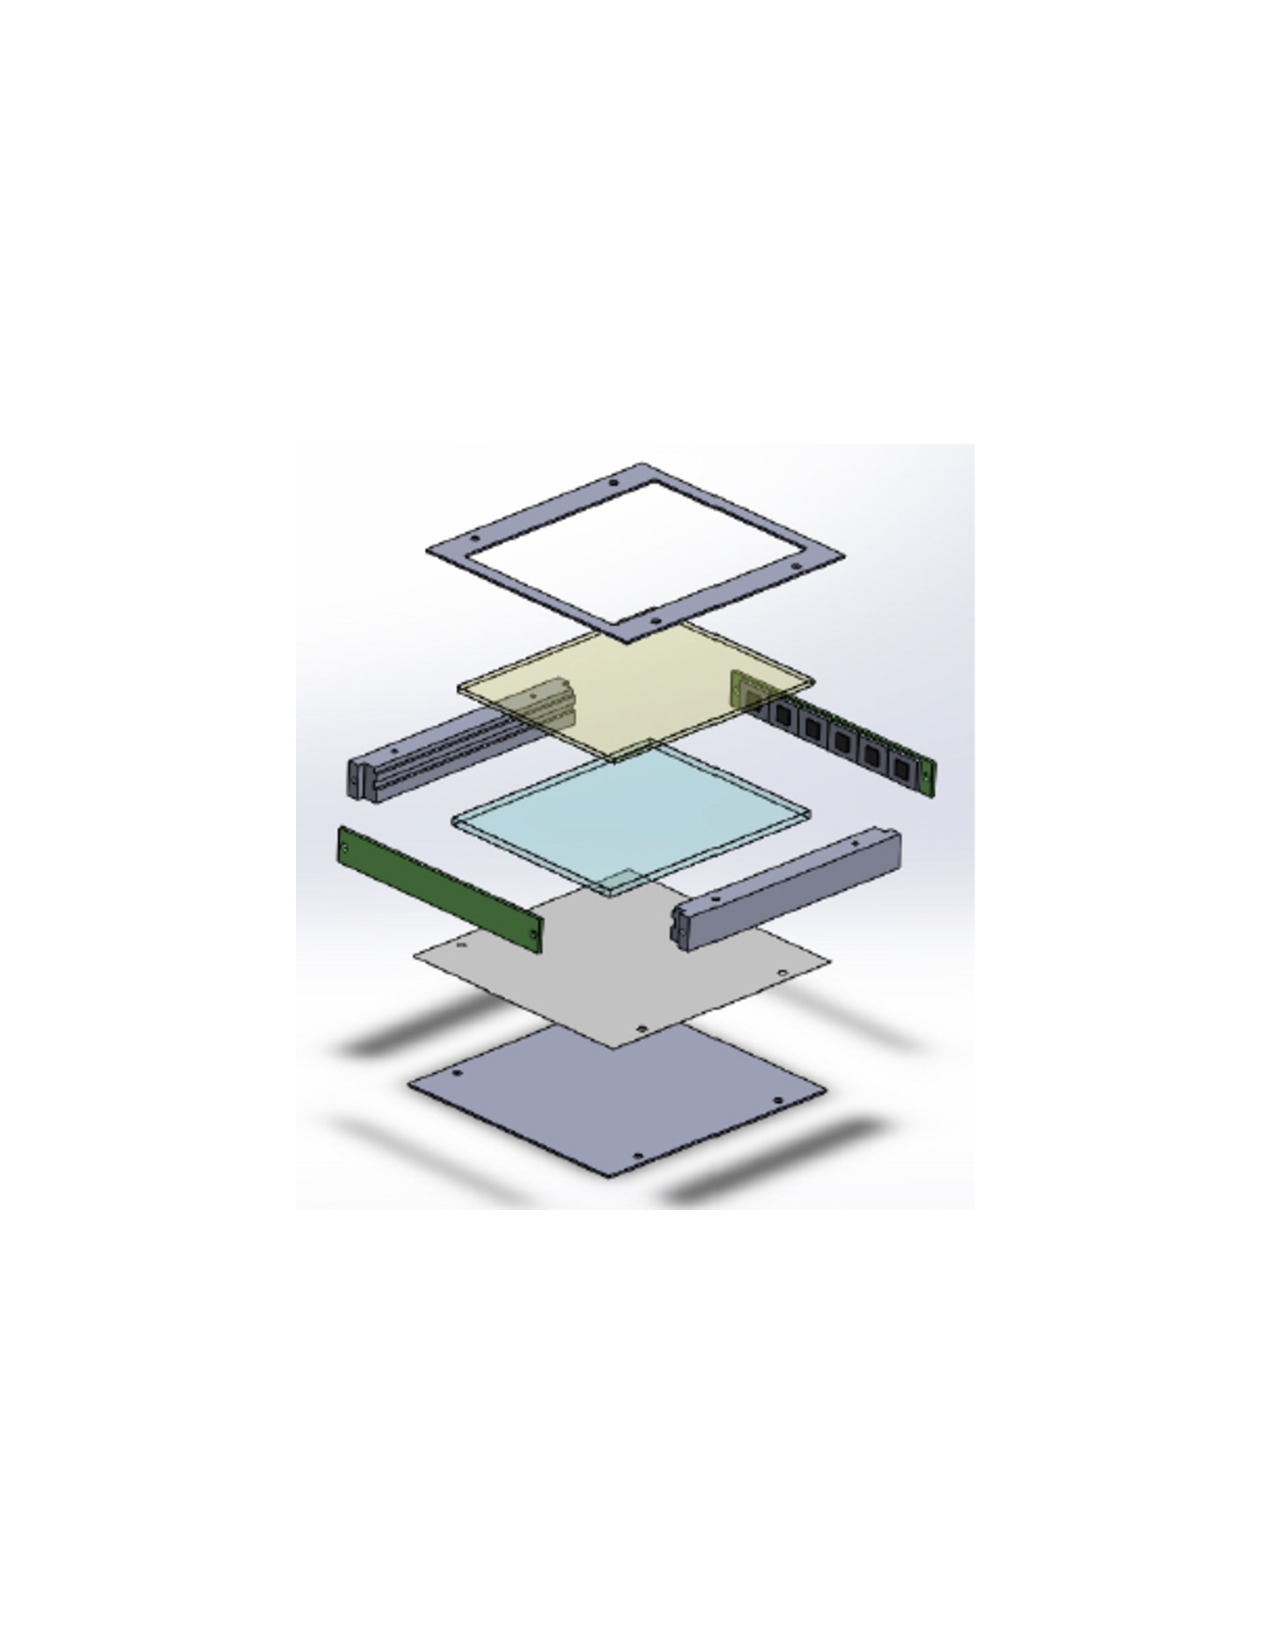
\includegraphics[height=.30\textheight]{pds-X-Arapuca-exploded-view.jpg}
\end{dunefigure}

% In a standard ARAPUCA the photon trapping effect is obtained by means of a dichroic filter and a two-steps wavelength shifting process, %the first from VUV to UV outside the acceptance window of the box and the second inside from UV to blue, across the filter cutoff. Double %shifted photons are eventually collected by an array of photosensors (SiPM) distributed on the backplane of the box, opposite to the the %acceptance window. 

In the X-ARAPUCA design, Figure \ref{fig:pds-x-arapuca-cell}, the inner shifter coating/lining over the reflective walls of the box is replaced by a thin wavelength-shifting light guide slab inside the box, of the same dimensions of the acceptance filter window and parallel to it. The SiPM arrays are installed vertically on the sides of the box, in optical contact to the light guide thin ends. 
 In this way a fraction of the photons will be converted inside the slab and guided to the read-out, other photons,  e.g. those at small angle of incidence below the critical angle of the light guide slab, after conversion at the slab surface will be remain trapped in the box and eventually collected as for the standard ARAPUCA.
 
 A full sized X-ARAPUCA prototype is under construction. The light guide is made by a 2 mm thick TPB doped acrylic slab. Specially designed read-out boards have been realized, made of 6 passively ganged SiPMs in a strip configuration.  Two boards into a single channel readout light signals from the X-ARAPUCA box. 
 
 %  V2 - text below aded to v1 - FC 22feb18 %%%%%%%%%%%%%%%%%%%%%%%%%%%%%%%%%%%
 A variant of the approach to the dipped-bar PD option described in the preceding section, 
 that might also have application in the X-ARAPUCA PD configuration,
 would be to use the now conventional extruded-scintillator process.  Standard extruded scintillator bar (like that
used in MINOS) has a core of polystyrene and a cladding of acrylic.  The core is doped with
a primary dopant (often p-terphenyl) and a wavelength shifter (WLS).  The cladding, in the case of
MINOS, was doped with a reflector, TiO$_2$.  For the DUNE PD system, the primary dopant would
be moved to the cladding and over-doped (3-5\% by wt.) and no reflector would be used.  The cladding polymer would be a
high-grade acrylic.  The polystyrene core would be doped with the desired WLS.   The very-high
doping level in the cladding would mean that p-terphenyl molecules would be separated by only 
$\simeq 1~\mathrm{\AA}$, so the p-terphenyl in the acrylic can effectively absorb the UV
photons.  A reflector layer could be added to the three faces not facing the LAr. 
The potential advantages of this variant are expected to be in a 
better uniformity, stability, well established and low-risk process, and cost.
%%%%%%%%%%%%%%%%%%%%%%%%%%%%%%%%%%%%%%%%%%%%%%%%%%
 

%==========================================================================================

\subsection{Photon Collector: Dip-Coated Light Guides}
\label{ssec:fdsp-pd-pc-bar1}
%\metainfo{\color{red} \bf Content needed: (4 pages) Toups}

\subsubsection{Description}

Figure~\ref{fig:pds-dippedbarpic} illustrates the process by which LAr scintillation photons are converted and detected by the dip-coated light guide bars.  VUV scintillation photons arriving at the bar are absorbed and wavelength-shifted to blue ($\sim430$ nm) by the TPB-based coating on the surface of the bar.  A portion of this light is captured in the bar and guided to one end through total internal reflection where it is detected by an array of SiPMs, whose PDE is well-match to the blue light.

\begin{dunefigure}[Schematic of light detection with dipped bars.]{fig:pds-dippedbarpic}
{Schematic of light detection with dipped bars.}
  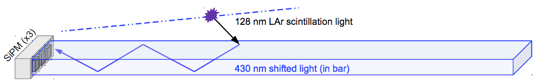
\includegraphics[width=0.8\columnwidth]{pds-dippedbarpic.png}
\end{dunefigure}

The dipping process and coating formula have undergone a series of development iterations~\cite{moss-2015},
%% this is illegal syntax
%\cite{Z. Moss et al 2015 JINST 10 P08017, Z. Moss et al 2016, arXiv:1604.03103v1}, 
which has led to the consistent production of light guide bars with measured attenuation lengths greater than 2~m. 

\subsubsection{Testing}

The dip-coated light guide bars have undergone extensive testing at both room and cryogenic temperatures.  As a part of the production process, the attenuation of each dip-coated light guide bar is measured at room temperature in a dark box with a UV LED.  In addition, some of these bars were also tested using $^{210}$Po alpha sources in the TallBo cryogenic test stand at FNAL~\cite{moss-2016}.
%% this is illegal syntax
%\cite{Z. Moss et al 2015 JINST 10 P08017, Z. Moss et al 2016}.  
These tests validated a model for predicting dip-coated light guide bar attenuation lengths in liquid argon based on measurements of attenuation lengths at room temperature, which are much easier to perform.  In addition, comparative tests of the dip-coated light guide bars and other candidate photon detector technologies for the DUNE single-phase far detector were performed in the TallBo cryostat at FNAL.

\subsubsection{Performance}

Tests of the dip-coated light guide bars in the TallBo cryostat with alpha sources indicate that the attenuation length of the bars in liquid argon is $>2$ m.  Data using tracked cosmic muons in TallBo indicated that the dip-coated bars have comparable or better performance than the other candidate photon detection technologies prototypes~\cite{whittington-2016}.
%% illegal syntax: \cite{D. Whittington 2016 JINST 11 C05019}.
Both of these tests are planned to be repeated in the near future.  In addition to extracting the attenuation length using an alpha source in TallBo, the overall efficiency will also be extracted by comparing the number of photoelectrons detected at the end of the bar to the number of photons from the alpha source impinging on the surface of the bar.

\subsubsection{Potential Improvements for the DUNE Far Detector}

There are two areas of potential improvements to the dip-coated light guide bars for the DUNE single-phase far detector: improving the coating performance and enhancing the readout of the light guide bars.  Regarding improvements to the coating performance, test bars have been produced with a higher TPB-to-acrylic ratio, which may have a higher conversion efficiency without sacrificing a reduction in attenuation length.  Regarding enhancing the readout of the light guide bars, one straightforward improvement under consideration is to read out both ends of the light guide bar rather than a single end as was done for the dip-coated bars deployed in ProtoDUNE-SP.  This improvement could increase the photon detection efficiency of the dip-coated light guide bars by up to a factor of two.

%==========================================================================================
\subsection{Photon Collector: Double-Shift Light Guides}
\label{ssec:fdsp-pd-pc-bar2}
%\todo{\color{blue} Content: Whittington}
%Update DW 2/23/18

The double-shift light guide photon collector design aims to maximize the active VUV-sensitive area of the photon detection system module while minimizing the necessary photocathode (SiPM) coverage. Commercially-fabricated plastic can be manufactured to transport light via total internal reflection with low attenuation losses. However, direct application of coatings to such manufactured optical surfaces can have an adverse impact on the effective attenuation length by introducing or exaggerating imperfections in the surface quality. To maintain the long intrinsic attenuation length of a manufactured light guide, the double-shift light guide design decouples the conversion of VUV photons to optical by arraying acrylic plates coated with TPB in front of a commercially-fabricated polystyrene light guide doped with a second wavelength-shifting compound.

\subsubsection{Description}

Figure~\ref{fig:pds-doubleshiftlg-cartoon} illustrates the process by which LAr scintillation photons are converted and detected by a double-shift light guide module. VUV scintillation photons impinging on the acrylic plates are converted to blue wavelengths. A portion of these blue photons penetrate the light guide and are converted to green. The isotropic re-emission of these green photons leads to a significant fraction becoming trapped by total internal reflection within the light guide. Trapped photons are transported to the end of the light guide where they are detected by an array of SiPMs.

\begin{dunefigure}[Schematic of the operation of a double-shift light guide.]{fig:pds-doubleshiftlg-cartoon}
{Schematic of the operation of a double-shift light guide.}
  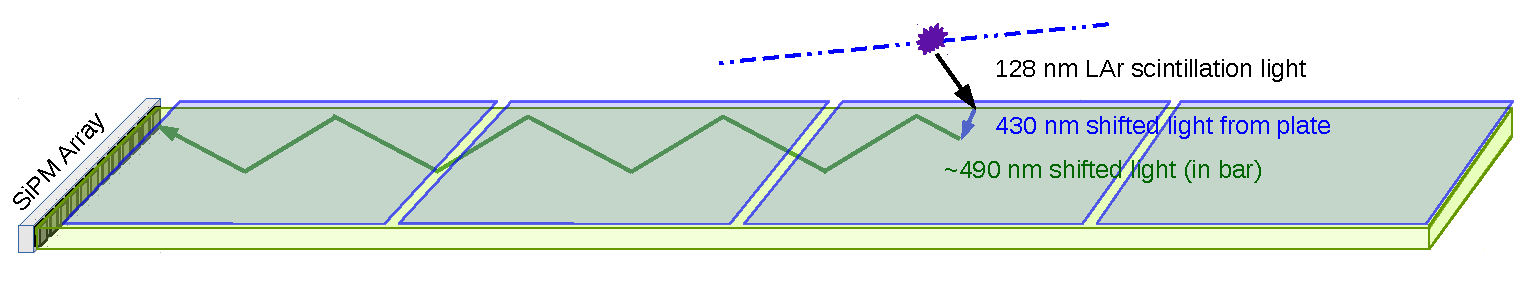
\includegraphics[width=0.8\columnwidth]{pds-doubleshiftlg-cartoon.pdf}
\end{dunefigure}


%\begin{itemize}
%\item Wavelength-Shifting Plates: Acrylic spray-coated with TPB. \fixme{TPB absorption and emission properties.}
%\item Wavelength-Shifting Light Guide: EJ-280 light guides manufactured by Eljen Technologies\footnote{http://%www.eljentechnology.com}. \fixme{EJ-280 absorption and emission properties. PDE of SiPMs.}
%\end{itemize}

\subsubsection{Wavelength-Shifting Plates}

The wavelength shifting compound tetraphenyl-butadiene\footnote{1,1,4,4-tetraphenyl-1,3-butadiene} (TPB) is commonly used to convert scintillation light from liquid noble elements to visible wavelengths. TPB emits visible photons typically between 420~nm and 450~nm. TPB is affixed to the outer surface of acrylic radiator plates suspended in front of the light guide. Six of these plates are mounted on each side of the light guide in a full-sized 210 $\times$ 8.6 cm$^2$ double-shift light collector module.

\subsubsection{Wavelength-Shifting Light Guide}

A portion of the photons emitted by the TPB radiator plates impinge on an EJ-280 light guide manufactured by Eljen Technologies\footnote{http://www.eljentechnology.com}. This is a commercially-fabricated polystyrene light guide doped with a second wavelength shifter. The EJ-280 wavelength shifter features an absorption spectrum that is well matched to the TPB emission spectrum. Absorbed photons are then re-emitted with typical green wavelengths in the range 480~nm to 510~nm.

\subsubsection{Photodetectors}

This double-shift light guide design has been developed using an array of SensL C-series\footnote{http://sensl.com/products/c-series/} MicroFC-60035-SMT SiPMs as the optical photocathode collecting converted light from the light guide. This model has a photon detection efficiency between 20\%--35\% across the emission spectrum of the EJ-280 wavelength shifter. This model of SiPM was chosen to match the emission spectrum of TPB, where it offers a $\sim$40\% efficiency, so improvement in the overall performance of this design can be achieved by selecting an alternate model with a better-matched photon detection efficiency.

\subsubsection{Testing}

The double-shift light guide design has undergone a series of development iterations to improve its performance, carried out at Indiana University (IU) and at Fermilab's cryogenic and vacuum test facility in the Proton Assembly Building (PAB). Comparative testing of light guide designs at PAB in mid-2015 demonstrated the double-shift light guide concept~\cite{bib:JINST-11-C05019}. An improved design similar to that deployed at ProtoDUNE-SP was studied at the Blanche test stand at Fermilab in September of 2016 with a complementary component-wise analysis program at IU afterward, detailed in Ref.~\cite{bib:DoubleShiftLG-NIM-171113}. The attenuation characteristics of this light guide were measured at IU while the global quantum efficiency for detecting incident LAr scintillation photons was measured with a vacuum-ultraviolet (VUV) monochromator at IU and using scintillation light from cosmic rays at the Blanche test stand.

\subsubsection{Performance}

Analysis of the double-shift light guide's attenuation properties determined an attenuation profile in LAr characterized by a double-exponential function of the form $f(z) = A \exp(-z/\lambda_{A}) + B \exp(-z/\lambda_B)$ with $z$ the distance from the instrumented end and parameters $A = $0.29, $\lambda_A = $4.3cm, $B = $0.71, and $\lambda_B = $225 cm~\cite{bib:DoubleShiftLG-NIM-171113}. The effective attenuation length is comparable to the width of an APA when the double-shift light guide is deployed in liquid argon.

Using both approaches the global quantum efficiency of this detector was determined to be 0.48\% at the readout end. The total effective area for detecting VUV scintillation photons can be determined by integrating the product of this global quantum efficiency and the attenuation function over the area of the detector:
\begin{equation*}
  A_{eff} = (0.0048) (8.5\text{cm}) \int_{0\text{cm}}^{210\text{cm}} \hspace{-2em}dz \left( 0.29 \exp(-z/4.3\text{cm}) + 0.71 \exp(-z/225\text{cm}) \right)
\end{equation*}
This corresponds to an effective area for detecting VUV scintillation photons of 4.1 cm$^{2}$ per module per drift volume. Six wavelength-shifting plates are deployed on each side of the light guide, meaning the double-shift light guide modules in the center APA array are sensitive to scintillation light from two drift volumes and modules in the outer arrays are able to detect scintillation light originating outside of the TPC volume.

%DWW 16mar18 start %%%%%%

%Moved from above dww�

\subsubsection{Potential Improvements for final design}

The double-shift light guide deployed in the ProtoDUNE-SP APAs was constrained to readout at a single end. Proposed changes to the APA size and cabling routing scheme for the DUNE single-phase far detector would allow for a second array of SiPMs at the opposite end of the light guide. This would double the performance of the photon detection system, raising the per-module effective area to 8.2 cm$^{2}$ per module per drift volume.

A SiPM with a wavelength-dependent PDE that is better matched to the EJ-280 emission spectrum would improve the overall efficiency. Simulations of the transport of light within the light guide suggest that applying a highly reflective coating to the long, narrow inactive sides of the light guide would further boost the attenuation function and increase the effective area of the light guide module. These effects combined lead to a potential increase of the effective area to 16 cm$^{2}$ per module per drift volume.

As is illustrated in Figure~\ref{fig:pds-sn-eff-simulation}, the simulated supernova neutrino detection capability of a photon detection system based on this %module depends strongly on small changes in the estimated efficiency. These potential improvements raise the physics performance in this channel into a %regime where small fluctuations in the module efficiency have a smaller impact on the efficiency to tag these supernova neutrino interactions. These %improvements are an important component to risk mitigation in the photon detection system performance.

%DWW 15mar18 end %%%%%%


%==========================================================================================

\subsection{Additional Techniques to Supplement or Enhance Light Yield}
\label{sec:fdsp-pd-enh}
%\metainfo{\color{blue} Content: Cavanna/Whittington/Machado}


%>> Start: Andrzej Szelc 14/02/2018 >>>>>>>>>>>>> 

\subsubsection{TPB-Coated Reflector Foils}
% Not a publication, but a proceedings:  To cite this article: Diego Garcia-Gamez and SBND Collaboration 2017 J. Phys.: Conf. Ser. 888 012094

Due to geometric effects, the baseline PDS design with photon detectors embedded within the APA frames will result
in a non-uniformity of light collection along the drift direction. Light emitted from interactions close to the APAs has an order of magnitude larger chance of being detected compared to interactions close to the CPA. This effect can be mitigated by installing wavelength-shifter (TPB) coated dielectric reflector foils on the cathode planes. Light impinging on these foils
can then be wavelength-shifted into visible wavelengths and reflected from the underlying foils. This light can subsequently be detected by photon detectors placed in the APAs provided they are sensitive to visible light. The primary result, 
shown in Fig. \ref{fig:ly_with_foils}, is the enhancement of the total light collection close to the cathode (black points), which will increase the detection efficiency in that region. 
Another benefit is the increase in uniformity - this can enable calorimetric reconstruction with scintillation light, which would enhance the charge-based energy reconstruction as well as increase the efficiency of triggering on low energy signals. Introducing the foils on the cathode can enable drift position resolution  using only scintillation light. This requires the photon detectors to be able to differentiate direct VUV light from re-emitted visible light( e.g. two different PD detector types) and good enough timing of arrival of first light.

Coated reflector foils are manufactured through low-temperature evaporation of TPB on dielectric reflectors e.g. 3M DM2000 or Vikuiti. Foils prepared in this manner have been successfully used in dark matter detectors \cite{warp}. Recently they have been shown to work in LArTPCs at neutrino energies, namely  in the LArIAT test-beam detector \cite{LArIAT}. In LArIAT they have been installed on the field-cage walls and, during the last run, on the cathode. This experience has led to the decision to install such foils on the CPA of the SBND detector. In DUNE, the foils would ideally be laminated on the CPA as well. However, because of the resistive CPA design, this requires additional R\&D to determine the fraction of the CPA area that could be covered with the dielectric foils.
This is an interface between the PDS and HV consortia. 

\begin{dunefigure}[Predicted light yield in a DUNE configuration after adding WLS-coated reflector foils.]{fig:ly_with_foils}
{Predicted light yield in a DUNE configuration after adding WLS-coated reflector foils. Blue points represent direct light impinging on the PDs, red stars - light wavelength-shifted and reflected on the CPA. Black points show total light yield.}
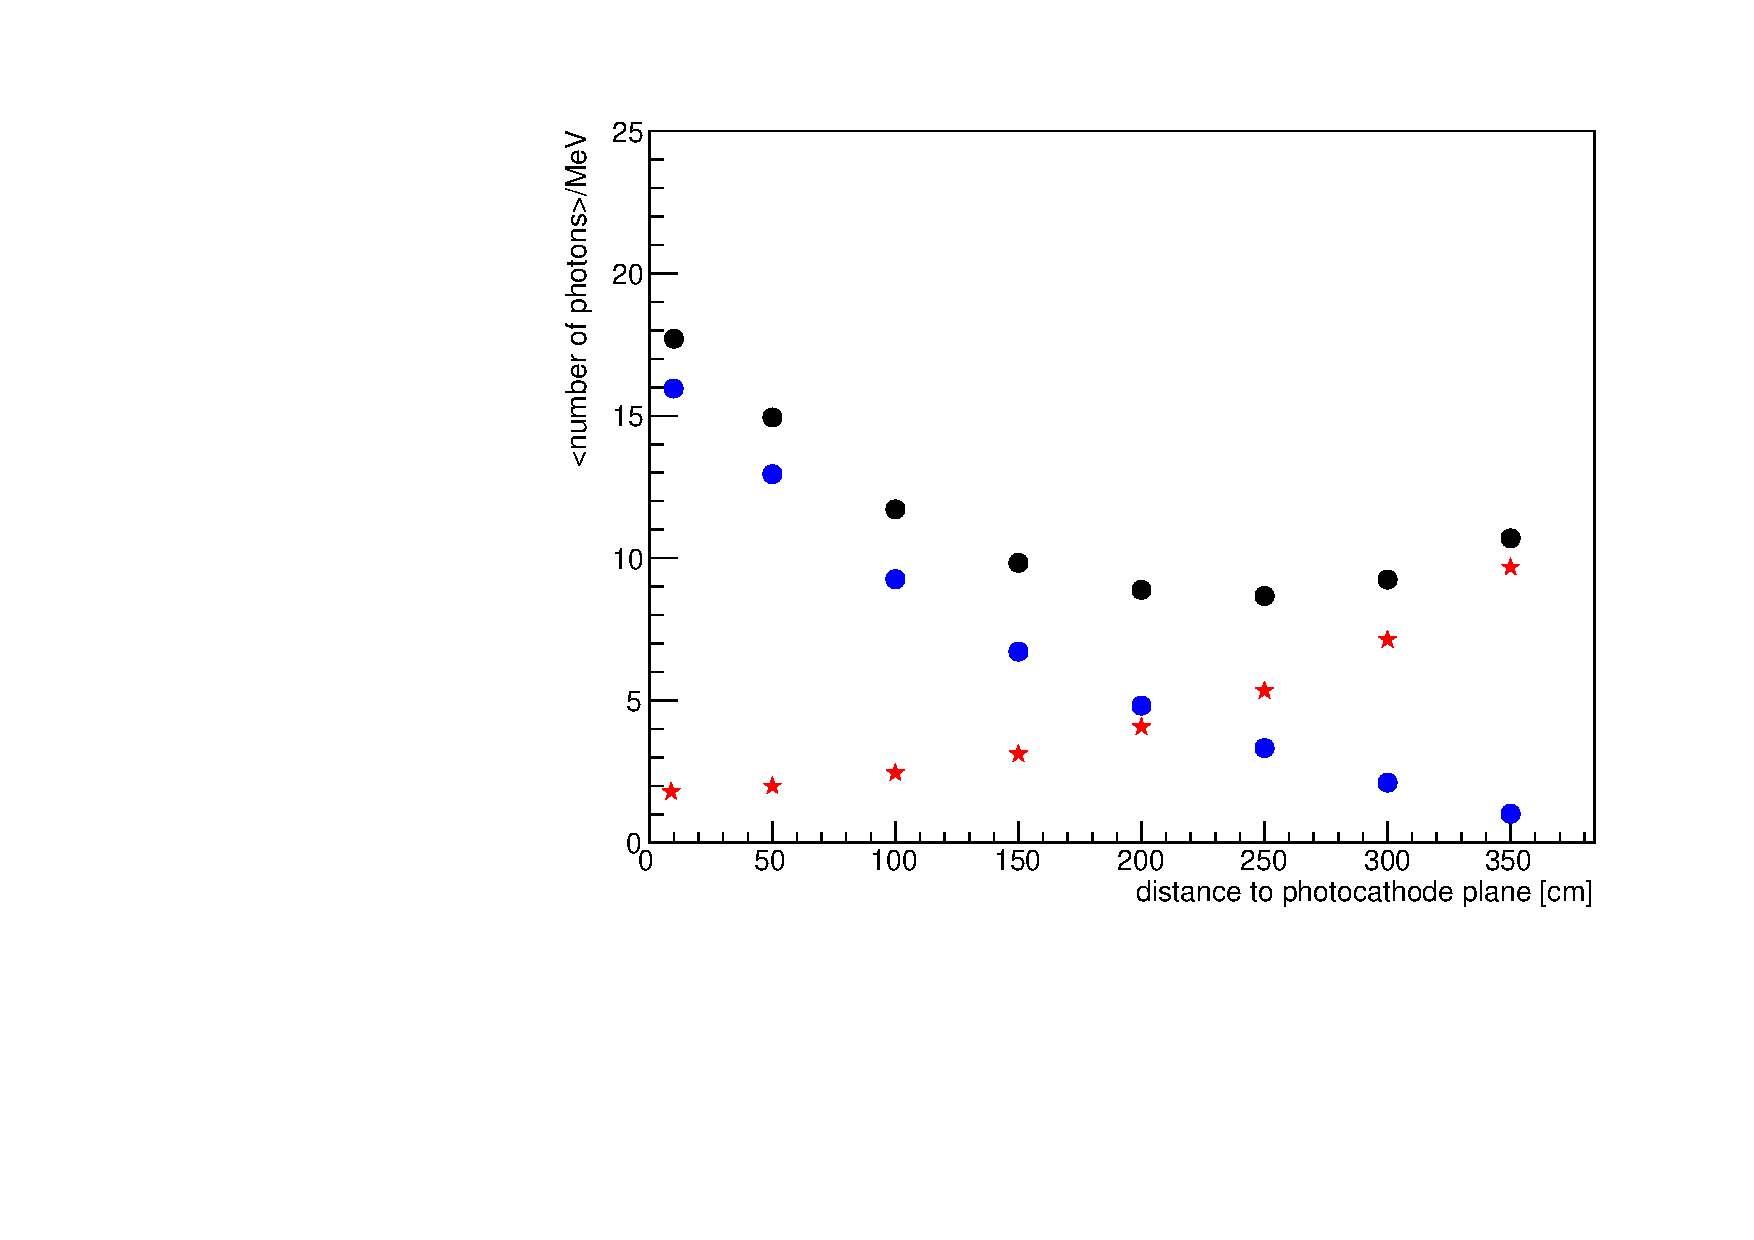
\includegraphics[width=0.5\columnwidth]{pds-ly_with_foils.pdf}
\end{dunefigure}

%<< Start: Andrzej Szelc 14/02/2018 <<<<<<<<<<<<<.

\subsubsection{Anode Plane Light Concentrators}
\label{sec:fdsp-pd-assy-lc}
%\todo{\color{blue} Content: Cavanna}
	
In the current baseline layout, the photosensitive area of the PD system is limited to about 12.5\% of the area of the anode plane - \todo{I am not sure what this means - rjw}delimiting one side of the LArTPC volume. 
Only a small fraction of the VUV direct light emitted in ionization events is thus intercepted by the photosensitive area, and this fraction also quickly reduces at increasing distance of the event from the anode plane.  Increase in light collection, both for the VUV and the reflected visible component (if the  TPB-coated foils at the cathode plane is adopted), can be achieved by implementing large area reflective surfaces at the anode plane (e.g. in the large open areas between PD bars inside the APA frames) acting as light concentrators toward the smaller photosensitive surfaces.  
This conceptual solution is suggested from the widely diffused implementation of Winston Cones for enhancing light collection in large volume liquid detectors. 
The PD bar geometry of the photosensitive area inside the thin APA frames and the related mechanical constraints impose rather severe limitations on the design - cone depth and entrance$/$exit apertures ratio - of the light concentrating surfaces. The installation of the reflective surfaces inside the APA frame would necessarily be made before wire winding. 
Ongoing studies are expected to demonstrate the feasibility of the solution and move the conceptual scheme into a technical design. MC simulations will determine the efficiency of the light concentrator. 
\fixme{it is difficult to picture what is intended without a figure}


%\subsubsection{Hybrid and New Options}

\subsubsection{Wavelength-Shifter Coated SiPM} 
The photon detectors described in the preceding section represent the results of a long process of optimization of the initial concepts developed years ago. A balance between the cost of the readout electronics (channel count), and the cost and performance of the SiPM's was achieved with realistic designs of the photon detectors offering the detection efficiency in the range $\sim$ 0.5 to 1.5\%.
 
A significant advances in the technology of the SPM's have been accomplished during this time: the photosensors dark count, after-pulsing and cross-talk rates have been lowered by almost an order of magnitude, whereas the production costs have been dropping significantly in response to the increasing range of applications.  The recent studies and tests demonstrate that the improved quality of the photodetectors is permitting much higher degree of ganging (passive or active), thus significantly lowering the "per SiPM" readout costs.
These technological trends are likely to continue, thus allowing for a possible alternative concepts of the photon detectors, even within the geometrical and cost confines of the baseline detectors.

One of the possible different concepts of the Photon Detector includes a long printed circuit board with the overall dimensions identical to the light guide bars or ARAPUCA but with a simpler construction involving only SiPMs distributed over the board surface. The SiPMs can be coated with  appropriate wavelength-shifter (TPB or MSB) or a foil with the wavelength-shifter in front of the SiPM can be used to convert the VUV 128 nm Argon light to the blue light at the maximum detection efficiency of the SiPM. The overall detection efficiency of such a ``detector element"is expected to be of the order of 25-30\%, depending on the pixel size and the fill-factor of the SiPM.

A photon detector involving the SiPMs only would offer a major simplification of the construction and integration efforts. Its overall performance can be reliably estimated and it is proportional to the total area of the bar covered with the SiPMs.
The performance of the baseline Photon Detectors can be achieved with 2-4\% of the area covered with the SiPMs. Taking 1800 cm$^2$ as a bar surface this coverage can be accomplished with 100-200 SiPMs of the standard 6x6 mm form factor. With 12-fold passive ganging, successfully demonstrated in recent tests, such a solution would require 8-16 readout channels per bar. The multiplexing level is limited by the noise of the readout electronics. Significantly higher degree of multiplexing can be achieved by use of larger pixel (e.g. 75x75 micron$^2$) SiPMs and/or possible cold active ganging circuitry. 
Such a detector concept appears very flexible and it would allows for future optimization in response to the expected technological advances with no or minimal impact on the rest of the DUNE  detector. 


%\paragraph*{Beyond the TDR} The Technical Proposal and TDR may include proposals to augment the capabilities of the photon
%collector modules. In the case that the hardware requirements for such proposals would pose a minimal
%impact on the detector design, additional R\&D beyond the timescale of the TDR may be required since it may impact the second 10~kt module if not the first. 
%Some examples include:
%\begin{itemize}
%\item TPB-Coated Reflector Foils %(Szelc)
%\item Xenon-Doped LAr %(Escobar/Para)
%\item TPB-Doped LAr %(Escobar)
%\end{itemize}

%%%%%%%%%%%%%%%%%%%%%%%%%%%%%%%%%%%

\subsection{Photon Sensors}
\label{sec:fdsp-pd-ps}
%\todo{\color{blue} Content: Zutshi}

The SP DUNE Photon Detector System uses a multi-step approach to scintillation light detection.  The first stage consists of large-area photon collectors that convert 128~nm (VUV) photons into the visible range (> 400~nm). Conversion into electrical charge, the {\it photon sensor}, is performed by much smaller
 silicon photomultipliers (SiPM) mated to the light collectors described earlier in this section. Robust photon detection efficiency, low operating voltages, small size and ruggedness make their usage attractive in the single phase design where the photon detectors must be accommodated inside the APA frames. 
As implemented in ProtoDUNE-SP, there are twelve \num{6}$\times$\num{6}\si{mm$^2$} SiPMs per bar and 6-12 per ARAPUCA box. With this configuration, a \SI{10}{kt} SP far detector with \num{150} APAs, each with \num{10} PD modules, would contain \num{18000}-\num{36000} (single or double-ended readout) SiPMs for the solid bars design and 10-20 times more for the higher granularity ARAPUCA design. This corresponds to approximately1-13~m$^2$ of active SiPM surface area.

In the following we summarize the most salient guiding principles and requirements for this SiPM-based photodetection system.

\begin{itemize}

\item Although developing the full suite of SiPM requirements (number of devices, dynamic range, triggering, 
zero-suppression threshold etc.) in light of the physics goals is an ongoing process, it is already clear
from the R$\&$D carried out to date that devices from several vendors have the 
performance characteristics in the vicinity needed for the DUNE photon detector
system (see Table~\ref{tab:photosensors}). A significant number of several types of these devices are being installed in 
ProtoDUNE-SP, which will provide an excellent test bed for evaluating and monitoring SiPM
performance in a realistic environment over the medium term.

\item A key requirement, based on past experience, is ensuring the mechanical and electrical 
integrity of these devices in a cryogenic environment. This is a requirement that 
catalog devices from most vendors do not satisfy as they typical are only certified for operation 
down to -40$^\circ$C. Thus it is of paramount importance to be in close communication with 
 vendors in the design, fabrication and SiPM packaging certification stages to ensure that the device will be robust and
reliable for long-term operation in a cryogenic environment. There is interest from at least two vendors (Hamamatsu and FBK) 
to engage with the Consortium in this fashion with the goal of having the vendor warrantying the product
for our application. Contact with other vendors and experiments (e.g. DarkSide) is being pursued.   

\item Comparative performance evaluation of promising SiPM candidates from
multiple vendors will need to be carried out in parallel over the next year. This evaluation will not only need to
address inherent characteristics (gain, dark rate, x-talk, after-pulsing etc) and ganging 
performance but also form factor, spectral response and mating with regard to the
multiple photon collector options. Experience acquired from ProtoDUNE-SP construction
and operation will inform QA/QC plans for the full detector, which will need to be
delineated in detail.

\item The optimal SiPM may depend on the photon collector option.  All photon collector
options currently being considered involve shifting the 128 nm LAr scintillation light to 
longer wavelengths, but each may present a different  spectral distribution to the SiPM. 
In this case, selection of the SiPM might wait to be optimally matched to the collector. 
However, we would not expect this fine-tuning to more than a 15-20\% effect, so it is not a driving factor.

\item The SiPM packaging should allow for tileable arrays to be constructed to facilitate high efficiency mating to the photon collectors and efficient space utilization inside the APA frame.

\item To reduce channel count, current size candidates SiPMs must be electrically ganged or fabricated in larger sizes. Electrical ganging (active or passive) is a joint responsibility of the Photon Sensor and Electronics working groups.

\item The SiPM signal path must be separate from the TPC readout. This implies that there must be cables dedicated to bringing the power
in and taking the analog or digitized signals from the PD system out of the cryostat. So, in addition to the desire for channel count reduction to reduce readout electronics cost, feedthrough cable space limitations will also imply some level of electrical ganging of the SiPM
signals inside the LAr volume. Investigation of this issue is being pursued in collaboration with the APA Consortium by the respective interface groups.
\end{itemize}

\begin{dunetable}[Candidate photosensors characteristics.]
%{lllll}
%{|p{0.2\textwidth}|p{0.2\textwidth}|p{0.2\textwidth}lp{0.2\textwidth}|p{0.2\textwidth}l}
{p{0.19\textwidth}p{0.19\textwidth}p{0.19\textwidth}p{0.19\textwidth}p{0.19\textwidth}}
{tab:photosensors}
{Candidate Photosensors Characteristics.}
	&Hamamatsu            & SensL                                  & KETEK                       & Advansid                      \\ \toprowrule
Series part \#       & S13360                                 & DS-MicroC                   & PM33                      & NUV-SIPMs                \\ \colhline
Vbr range            & 48 V to 58 V                             & 24.2 V to 24.7 V              & 27.5 V                     & 24 V to 28 V               \\ \colhline
Vop range            & Vbr + 3 V                               & Vbr +1 V to +3 V              & Vbr+2V to +5 V             & Vbr +2 V to +6 V           \\ \colhline
Temp. dependence     & 54 mV/K                                & 21.5 mV/K                    & 22 mV/K                    & 26 mV/K                   \\ \colhline
gain                 & $1.7 \times 10^6$                  & $3 \times 10^6$            & $1.74 \times 10^6$      & $3.6 \times 10^6$ \\ \colhline
pixel size           & 50 $\mu$m                          & 10 $\mu$m to 50 $\mu$m       & 15 $\mu$m to 25 $\mu$m     & 40 $\mu$m           \\ \colhline
sizes                & 2x2 mm                                  & 1x1                         & 3x3                       & 4x4                      \\ \colhline
                     & 3x3 mm                                  & 3x3                         &                           & 3x3                      \\ \colhline
                     & 6x6 mm                                  & 6x6                         &                           &                          \\ \colhline
wavelength           & 320 to 900 nm                           & 300 to 950 nm                & 300 to 950 nm              & 350 to 900 nm             \\ \colhline
PDE peak wavelength  & 450 nm                                  & 420 nm                       & 430 nm                     & 420 nm                    \\ \colhline
PDE @ peak           & 40\%                                   & 24\% to 41\%                & 41\% at Vov=5 V           & 43\%                     \\ \colhline
DCR @0.5PE           & 2 to 6 MHz                             & 0.3 kHz to 1.2 MHz             & 100 kHz  at Vovr=5 V         & 100 kHz/mm$^2$              \\ \colhline
Crosstalk            &                                        & 7\%                         & 15\%                      &                          \\ \colhline
Afterpulsing         &                                        & 0.20\%                      & \textless 1\%             & \textless4\%             \\ \colhline
Terminal capacitance & 1300 pF                                 & 3400 pF                      & 750 pF                    &800 pF                                     \\ \colhline
Lab experience       & Good experiences from Mu2e and ARAPUCA & Crack at LN2 temps. after specifications change&                 &     \\         
\end{dunetable}


%%%%%%%%%%%%%%%%%%%%%%%%%%
%The planned photodetector is a SiPM, model 
%SensL C-Series 6~mm$^2$
%(MicroFB-60035-SMT). % device. 
%This model of SiPM has a detection efficiency of
%41\%; the quoted detection efficiency incorporates Quantum Efficiency (QE) and 
%the effective area
%  coverage accounting for dead space between pixels.   At LAr temperature (89~K) the dark rate is of order 10~Hz
%(0.5 p.e. threshold), and  after-pulsing has not been observed. An on-going testing program is in place to ensure 
%that the SiPMs can reliably survive the stresses associated with 
%any thermal cycling in LAr and long-term operation at LAr temperature.

%All photodetectors %for ProtoDUNE-SP 
%are subjected to testing to determine
 %forward and reverse bias I-V curves,
 %breakdown voltage, dark current and dark count rate, photodetector gain, crosstalk estimation, response, and bias dependence of parameters.
 
%All SiPMs 
%Each SiPM is tested before mounting on the readout boards to determine
%if the part meets the specifications in a warm test.  After mounting to
%the readout board all items are tested both warm and cold (cyrogenic 
%temperature) to determine the operating characteristics.

%In addition to these tests, the photodetectors are tested for their
%response to light signals from an LED of appropriate wavelength.
%These tests will be sensitive enough to determine if one of the three SiPM
%elements operating in parallel is not functioning.


%%%%%%%%%%%%%%%%%%%%%%%%%%%%%%%%%%%
\subsection{Electronics}
\label{sec:fdsp-pd-pde}
%\metainfo{\color{red}\bf  Content: (3 pages) - Djurcic/Franchi/Moreno}

\subsubsection{Introduction}

%DWW 16mar18 start %%%%%%

% I am re-doing all this…

%The photon-detector design requires the readout system to collect and process electric signal from photo-sensors in liquid argon, 
%to provide interface with trigger and timing systems to support data reduction and classification, and to enable data transfer 
%to an offline storage for physics analysis.

%The photon-readout is required to enable the detector measurement of the time-zero of non-beam events with deposited 
%energy above \SI{200}{MeV}. This capability will also enhance beam physics, by recording interaction time of events within 
%beam spill to help separate against potential cosmic background interactions. In addition, any consideration of pulse-shape 
%discrimination will require capability to record both prompt and delayed components of scintillation light, latter one consisted mostly 
%from single photo-electrons at readout end. Photon-detector collects a limited amount of light, so it could be beneficial to 
%collect the light from both excited states. Therefore, important physics questions that may affect the design of the electronics 
%readout system include understanding of required time resolution for the photon readout system, and clarification whether 
%the system needs to efficiently collect single photo-electron signals. 

%Simplification in the readout scheme and a cost reduction will come from reading arrays of SiPMs, rather than individual 
%photo-sensors. To that end we desire a system where the single SiPM array reads a whole photodetector unit.
%Technical factors that affect performance of the system are type of the selected SiPM with characteristic capacitance, 
%number of SiPMs connected together with a choice of "ganging" scheme, to dictate signal to noise ratio and affect the system 
%performance and design considerations. Selection of the ganging option will include passive or active solutions, where the active 
%circuitry may require cold components such as an amplifier in LAr volume. Design options with active cold components will need 
%to address issues of power dissipation and potential risks of single-point failures of multi-channel devices inside the cryostat.
%In the case of passive ganging, analog signals are transmitted outside of the cryostat for processing and digitalization. 

%In general arrival time and total charge are the parameters to be obtained from a detector. Extraction of these parameters 
%is possible using analog or digital systems. Charge preamplifier is usually connected to the output of the detector to integrate 
%current producing a charge proportional output. In the case of digital systems an amplifier is needed to adjust the detector output signal 
%level to the input of an Analog to Digital Converter.  In both systems, performance parameters related  to sampling rate, number of bits, 
%power requirements, signal to noise ratio, and interface requirements should be evaluated to arrive to selected solution.  
%Pulse shapes can be fully analyzed to improve detection of a new physics but it will have an important impact on the digitalization %frequency.

The photon-detector design requires the readout system to collect and process electric signals from photo-sensors reading out the light collector bars, 
to provide interface with trigger and timing systems to support data reduction and classification, and to enable data transfer 
to an offline storage for physics analysis.

The photon-readout is required to enable the detector measurement of the time-zero of non-beam events with deposited 
energy above \SI{200}{MeV}. This capability will also enhance beam physics, by recording interaction time of events within 
beam spill to help separate against potential cosmic background interactions. Two main methods of data collection are currently considered:  self-triggered integrated charge readout and wave form digitization.  Charge integration appears to be a likely candidate at this point in our development, as it offers the potential for a simpler, commercially available charge integration circuit and perhaps a smaller, less-expensive cable plant to read it out.  Physics simulation studies are currently underway to determine if pulse-shape 
discrimination will be required, which would provide the capability to record both prompt and delayed components of scintillation light, latter one consisting mostly 
of single photo-electrons and thus place stringent requirements on signal-to-noise performance. The photon detector collects a limited amount of light, so it could be beneficial to 
collect the light from both excited states. Therefore, important physics questions that may affect the design of the electronics 
readout system include understanding of required time resolution for the photon readout system, and clarification whether 
the system needs to efficiently collect single photo-electron signals. 

Simplification in the readout scheme and a cost reduction can also be realized by reading arrays of SiPMs, rather than individual 
photo-sensors. Indeed, all of the SiPM mounting schemes involve some degree of active (cold amplification and signal summing) or passive ganging.  To that end we desire a system where the ganging is maximized to minimize electronics count while maintaining adequate redundancy and granularity, as well as readout system performance.  This represents a significant interface between the electronics, photo sensor and light collector designs, and will be a main focus of our development and optimization work up to the TDR.
Technical factors that affect performance of the ganging system are type of the selected SiPM with characteristic capacitance, 
number of SiPMs connected together, which can dictate signal to noise ratio and affect the system 
performance and design considerations. Selection of the ganging option will include passive or active solutions, where the active 
circuitry may require cold components such as an amplifier in LAr volume. Design options with active cold components will need 
to address issues of power dissipation and potential risks of single-point failures of multi-channel devices inside the cryostat.
In the case of passive ganging, analog signals are transmitted outside of the cryostat for processing and digitalization. 

In general arrival time and total charge are the parameters to be obtained from a detector. Extraction of these parameters 
is possible using analog or digital systems. Charge preamplifiers will be connected to the output of the detector to integrate 
current producing a charge proportional output. In the case of digital systems an amplifier is needed to adjust the detector output signal 
level to the input of an Analog to Digital Converter.  In both systems, performance parameters related  to sampling rate, number of bits, 
power requirements, signal to noise ratio, and interface requirements should be evaluated to arrive to selected solution.  
Pulse shapes can be fully analyzed to improve detection of a new physics but it will have an important impact on the digitalization frequency.

%DWW 16mar18 end %%%%%%

\subsubsection{ProtoDUNE-SP Experience}

As already described above the photon-detector development has matured to the point where three different photon-detector designs are 
prepared for ProtoDUNE-SP experiment at CERN, to be operational in the second half of \num{2018}. 
% For the bar-style photon-detectors the solution with three SiPM ganged together, being read-out through the single readout channels has been implemented. 
A dedicated photon-detector readout system with a high-performant electronics front-end was developed for the ProtoDUNE-SP experiment, 
as schematically presented in Figure~\ref{fig:fig-pds-readout}, left. A passive ganging scheme was chosen, where three SiPMs are ganged together.  
The un-amplified analog signals from the SiPMs are transmitted directly to outside the cryostat for processing and digitization. A custom module, 
called the SiPM Signal Processor (SSP), receives the SiPM signals outside the cryostat. An SSP consists of \num{12} readout channels packaged in 
a self-contained 1U module. Four SSPs are shown in Figure~\ref{fig:fig-pds-readout}, right. Each channel contains a fully-differential voltage 
amplifier and a \num{14}-bit, \num{150}-MSPS analog-to-digital converter (ADC) that digitizes the waveforms received from the SiPMs. The front-end amplifier 
is configured as fully-differential, and receives the SiPM signals into a termination resistor that matches the characteristic impedance of the signal cable. 

%\begin{dunefigure}[Block diagram of the ProtoDUNE-SP SSP module]{PD_fig-e-3}{Block diagram of the ProtoDUNE-SP SSP module} 
%\includegraphics[width=\textwidth]{pds-ProtoDUNE-SP-SSP-block-diagram.png}
%\end{dunefigure}

 \begin{dunefigure}[ProtoDUNE-SP Photon Detector readout.]
 {fig:fig-pds-readout}
 {Block diagram of the ProtoDUNE-SP photon detector readout module (left figure). Photon detector readout system operational at ProtoDUNE-SP (right figure). }
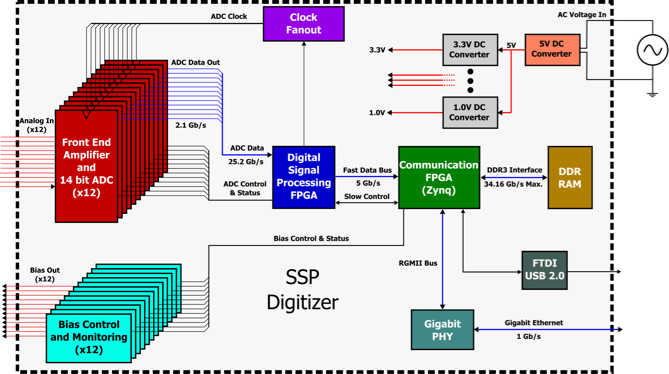
\includegraphics[angle=0,width=8.4cm,height=6cm]{pds-fig-e-3.png}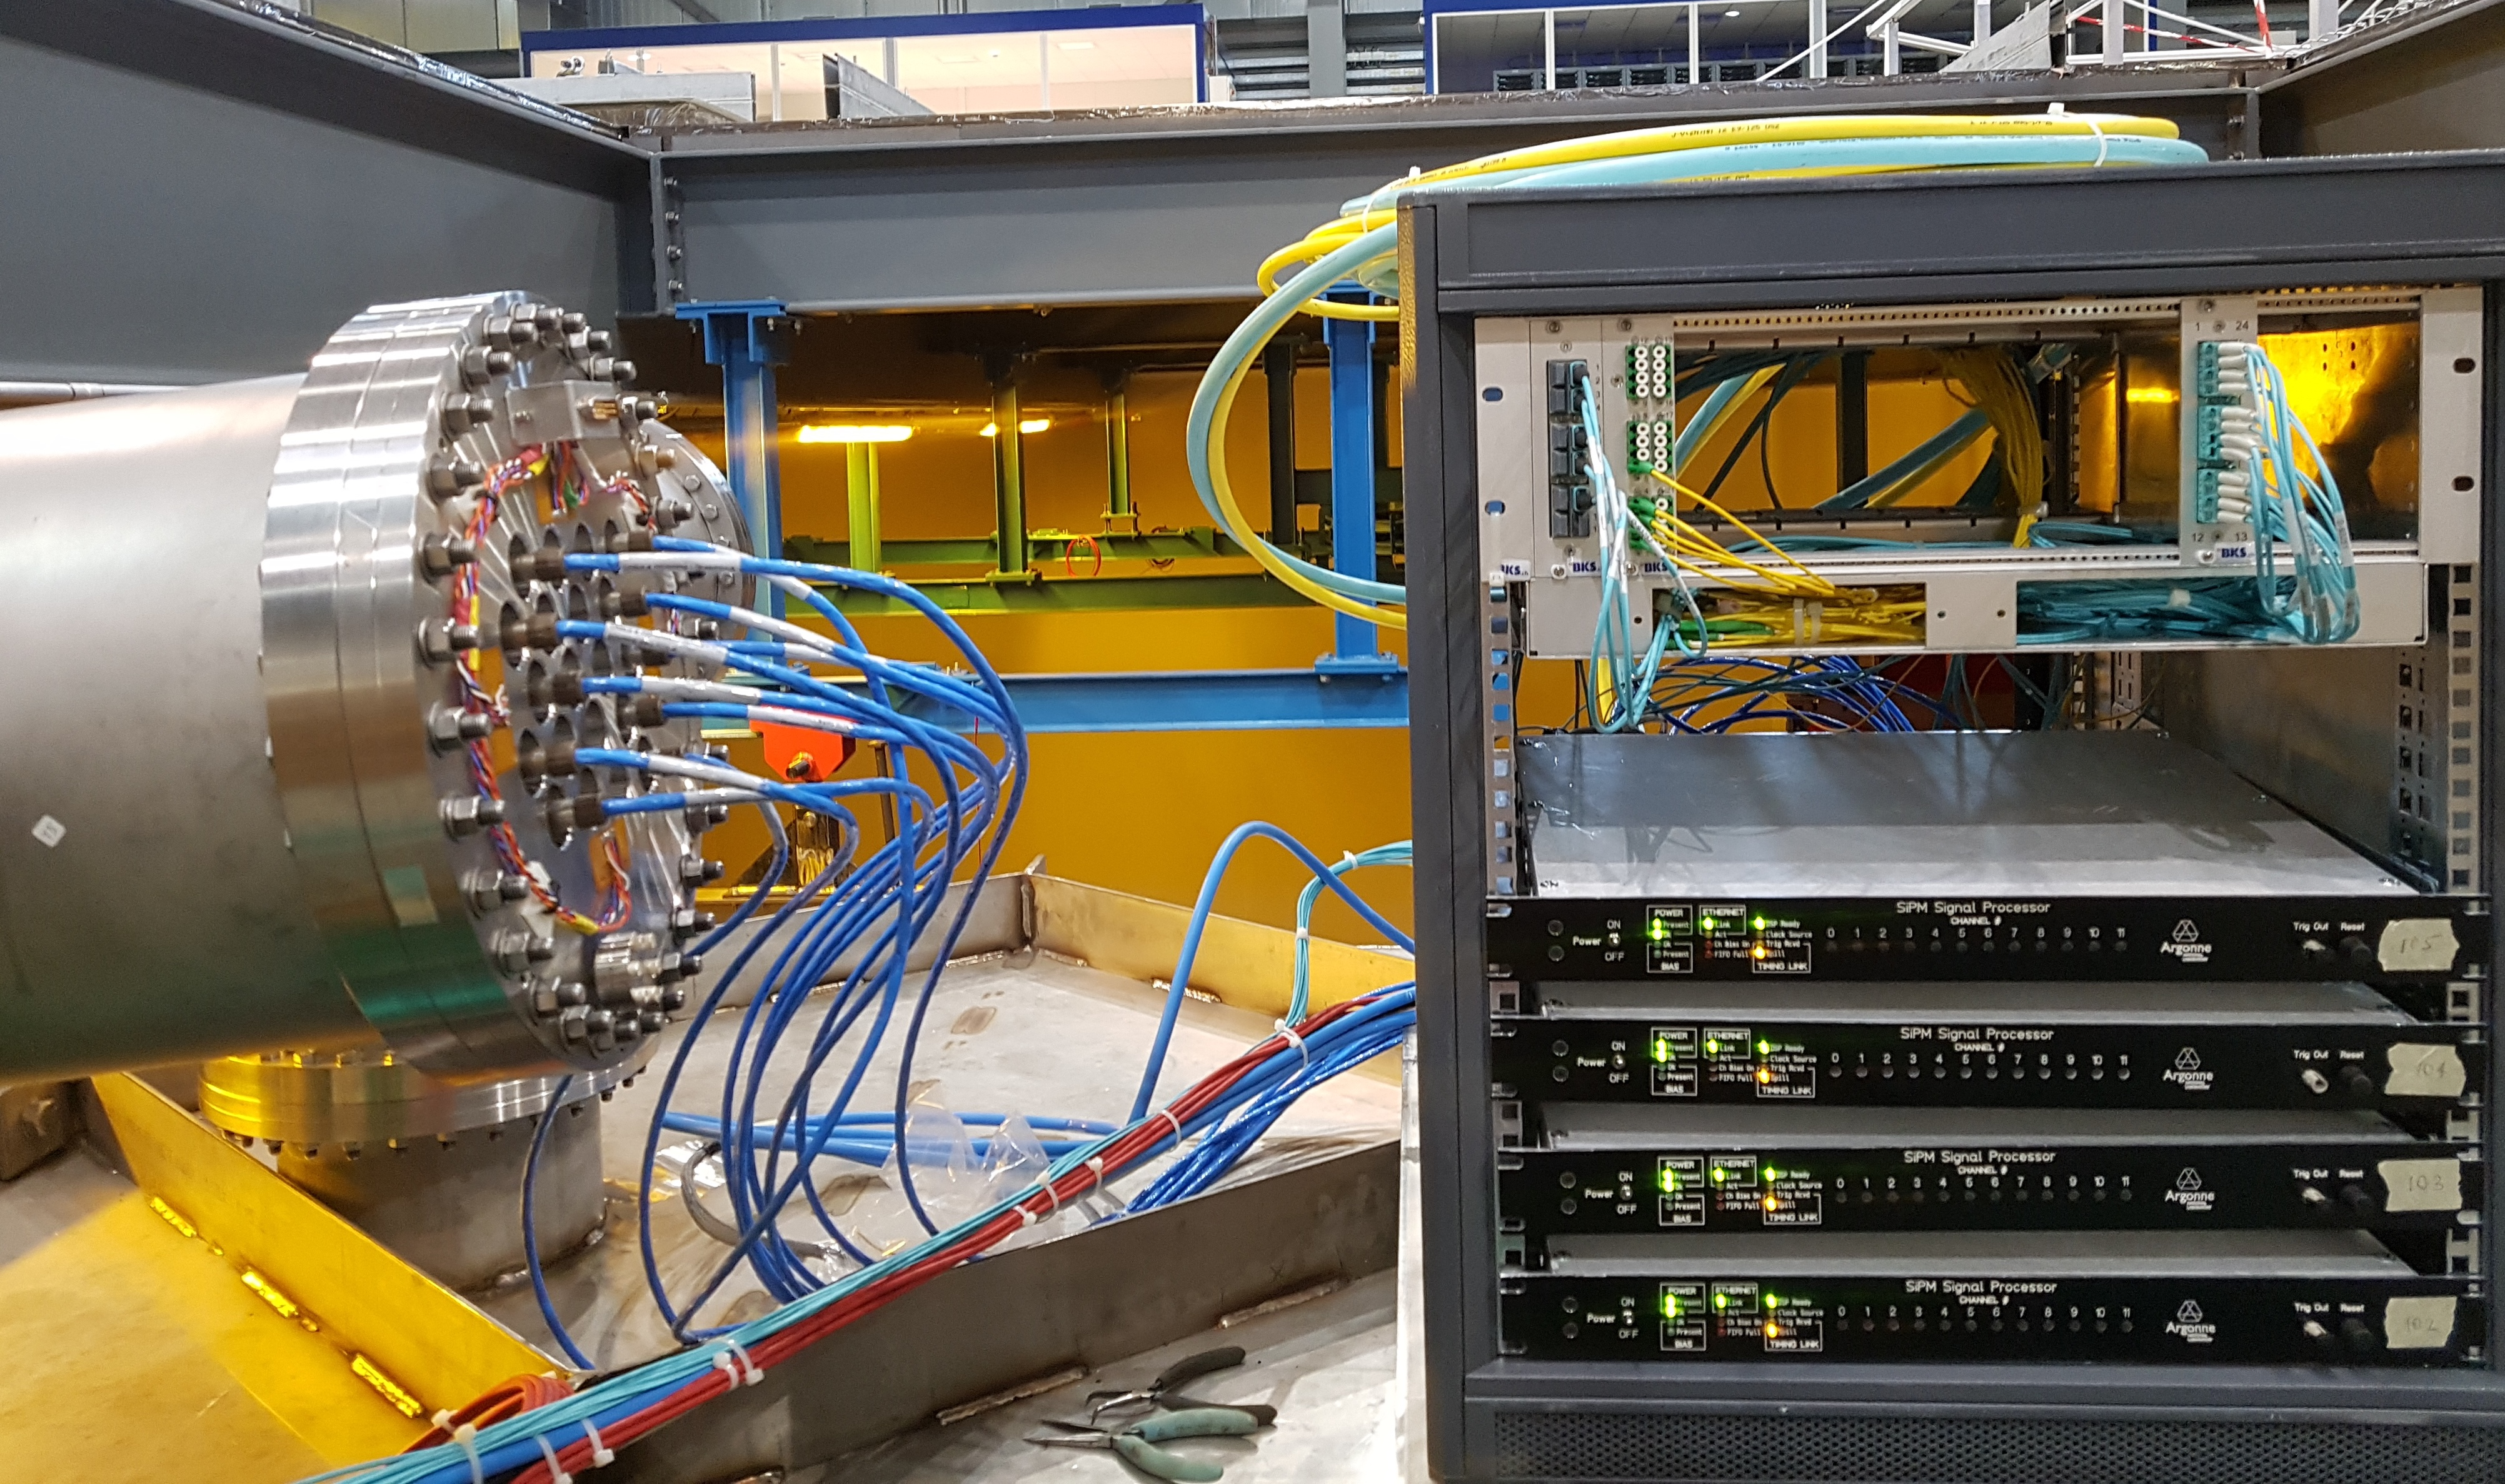
\includegraphics[angle=0,width=8.4cm,height=6cm]{pds-protodune_readout_coldbox.jpg}
\end{dunefigure}

In the standard mode of operation, the module performs waveform capture, using either an external or internal trigger. In the latter case the 
module self-triggers to capture only waveforms with an amplitude greater than a specified threshold. In the ProtoDUNE-SP the photon readout 
is configured to read waveforms when triggered by a beam event, and/or to provide header information when self-triggered by cosmic muons.
The header portion summarizes pulse amplitude, integral, and time-stamp information of events. The SSP for ProtoDUNE-SP uses \si{Gb} Ethernet 
communication implemented over an optical interface. The \SI{1}{Gb/s} Ethernet supports full TCP/IP protocol.  

The module includes a separate \num{12}-bit high-voltage DAC for each channel to provide bias to each SiPM. The SSP provides a trigger output signal 
from internal discriminators in firmware based on programmable coincidence logic, with a standard ST fiber interface to the central trigger board (CTB).
Input signals are provided to CTB from the beam instrumentation, the SSPs, and the beam TOF system. The CTB receives timing information from 
the ProtoDUNE-SP timing system and the CTB trigger inputs are distributed to the experiment via the timing system.
To that end the SSP implements the timing receiver/transmitter endpoint hardware to receive trigger inputs and clock signals from the timing system.


\subsubsection{Next Steps}

ProtoDUNE-SP test beam and cosmic-ray muon data analysis will provide evaluation of the readout system implemented in ProtoDUNE-SP.
Input from photon-detector photo-sensor and simulation groups, along with ProtoDUNE-SP input,  will provide important guidance on
how to optimize design and cost for DUNE Far Detector.

Additional development program requires us to optimize the ganging scheme with optimal choice of SiPM and cable types. With above inputs 
the choice between waveform readout and integrated charge readout will be made by taking into account DAQ communication and data 
readout requirements. The readout design will require understanding of physics requirements on time resolution, light yield 
sensitivity, with choices of photo-sensor type and ganging scheme. 

Time resolution must be stated by the physics requirements so the sampling rate and number of sample bits can be estimated. For this task 
some digital process such as a sample interpolation can be proposed, enhancing precision of the recorded raw sample time precision.

The light sensitivity and the dynamic range must also be based on physics goals. This decision will enable the number of bits and the sample 
rate required by either waveform or charge collection methods. In both cases the signal to noise ratio and the power consumption must be estimated. 
Two considered options could be then compared to model the final readout system where the choice is  correlated with the nature of ganging process. 
Charge processing requires a charge preamplifier ideally located within the cold environment, taking into consideration the failure risks and the power 
dissipated into the environment.

The design will be based on selected SiPM sensor and defined cable type, required event sampling rate, signal range expressed 
through number of sample bits, power requirements, signal to noise ratio, DAQ infrastructure, and optimized cost.


